% Options for packages loaded elsewhere
\PassOptionsToPackage{unicode}{hyperref}
\PassOptionsToPackage{hyphens}{url}
%
\documentclass[
]{article}
\usepackage{amsmath,amssymb}
\usepackage{iftex}
\ifPDFTeX
  \usepackage[T1]{fontenc}
  \usepackage[utf8]{inputenc}
  \usepackage{textcomp} % provide euro and other symbols
\else % if luatex or xetex
  \usepackage{unicode-math} % this also loads fontspec
  \defaultfontfeatures{Scale=MatchLowercase}
  \defaultfontfeatures[\rmfamily]{Ligatures=TeX,Scale=1}
\fi
\usepackage{lmodern}
\ifPDFTeX\else
  % xetex/luatex font selection
\fi
% Use upquote if available, for straight quotes in verbatim environments
\IfFileExists{upquote.sty}{\usepackage{upquote}}{}
\IfFileExists{microtype.sty}{% use microtype if available
  \usepackage[]{microtype}
  \UseMicrotypeSet[protrusion]{basicmath} % disable protrusion for tt fonts
}{}
\makeatletter
\@ifundefined{KOMAClassName}{% if non-KOMA class
  \IfFileExists{parskip.sty}{%
    \usepackage{parskip}
  }{% else
    \setlength{\parindent}{0pt}
    \setlength{\parskip}{6pt plus 2pt minus 1pt}}
}{% if KOMA class
  \KOMAoptions{parskip=half}}
\makeatother
\usepackage{xcolor}
\usepackage[margin=1in]{geometry}
\usepackage{color}
\usepackage{fancyvrb}
\newcommand{\VerbBar}{|}
\newcommand{\VERB}{\Verb[commandchars=\\\{\}]}
\DefineVerbatimEnvironment{Highlighting}{Verbatim}{commandchars=\\\{\}}
% Add ',fontsize=\small' for more characters per line
\usepackage{framed}
\definecolor{shadecolor}{RGB}{248,248,248}
\newenvironment{Shaded}{\begin{snugshade}}{\end{snugshade}}
\newcommand{\AlertTok}[1]{\textcolor[rgb]{0.94,0.16,0.16}{#1}}
\newcommand{\AnnotationTok}[1]{\textcolor[rgb]{0.56,0.35,0.01}{\textbf{\textit{#1}}}}
\newcommand{\AttributeTok}[1]{\textcolor[rgb]{0.13,0.29,0.53}{#1}}
\newcommand{\BaseNTok}[1]{\textcolor[rgb]{0.00,0.00,0.81}{#1}}
\newcommand{\BuiltInTok}[1]{#1}
\newcommand{\CharTok}[1]{\textcolor[rgb]{0.31,0.60,0.02}{#1}}
\newcommand{\CommentTok}[1]{\textcolor[rgb]{0.56,0.35,0.01}{\textit{#1}}}
\newcommand{\CommentVarTok}[1]{\textcolor[rgb]{0.56,0.35,0.01}{\textbf{\textit{#1}}}}
\newcommand{\ConstantTok}[1]{\textcolor[rgb]{0.56,0.35,0.01}{#1}}
\newcommand{\ControlFlowTok}[1]{\textcolor[rgb]{0.13,0.29,0.53}{\textbf{#1}}}
\newcommand{\DataTypeTok}[1]{\textcolor[rgb]{0.13,0.29,0.53}{#1}}
\newcommand{\DecValTok}[1]{\textcolor[rgb]{0.00,0.00,0.81}{#1}}
\newcommand{\DocumentationTok}[1]{\textcolor[rgb]{0.56,0.35,0.01}{\textbf{\textit{#1}}}}
\newcommand{\ErrorTok}[1]{\textcolor[rgb]{0.64,0.00,0.00}{\textbf{#1}}}
\newcommand{\ExtensionTok}[1]{#1}
\newcommand{\FloatTok}[1]{\textcolor[rgb]{0.00,0.00,0.81}{#1}}
\newcommand{\FunctionTok}[1]{\textcolor[rgb]{0.13,0.29,0.53}{\textbf{#1}}}
\newcommand{\ImportTok}[1]{#1}
\newcommand{\InformationTok}[1]{\textcolor[rgb]{0.56,0.35,0.01}{\textbf{\textit{#1}}}}
\newcommand{\KeywordTok}[1]{\textcolor[rgb]{0.13,0.29,0.53}{\textbf{#1}}}
\newcommand{\NormalTok}[1]{#1}
\newcommand{\OperatorTok}[1]{\textcolor[rgb]{0.81,0.36,0.00}{\textbf{#1}}}
\newcommand{\OtherTok}[1]{\textcolor[rgb]{0.56,0.35,0.01}{#1}}
\newcommand{\PreprocessorTok}[1]{\textcolor[rgb]{0.56,0.35,0.01}{\textit{#1}}}
\newcommand{\RegionMarkerTok}[1]{#1}
\newcommand{\SpecialCharTok}[1]{\textcolor[rgb]{0.81,0.36,0.00}{\textbf{#1}}}
\newcommand{\SpecialStringTok}[1]{\textcolor[rgb]{0.31,0.60,0.02}{#1}}
\newcommand{\StringTok}[1]{\textcolor[rgb]{0.31,0.60,0.02}{#1}}
\newcommand{\VariableTok}[1]{\textcolor[rgb]{0.00,0.00,0.00}{#1}}
\newcommand{\VerbatimStringTok}[1]{\textcolor[rgb]{0.31,0.60,0.02}{#1}}
\newcommand{\WarningTok}[1]{\textcolor[rgb]{0.56,0.35,0.01}{\textbf{\textit{#1}}}}
\usepackage{longtable,booktabs,array}
\usepackage{calc} % for calculating minipage widths
% Correct order of tables after \paragraph or \subparagraph
\usepackage{etoolbox}
\makeatletter
\patchcmd\longtable{\par}{\if@noskipsec\mbox{}\fi\par}{}{}
\makeatother
% Allow footnotes in longtable head/foot
\IfFileExists{footnotehyper.sty}{\usepackage{footnotehyper}}{\usepackage{footnote}}
\makesavenoteenv{longtable}
\usepackage{graphicx}
\makeatletter
\def\maxwidth{\ifdim\Gin@nat@width>\linewidth\linewidth\else\Gin@nat@width\fi}
\def\maxheight{\ifdim\Gin@nat@height>\textheight\textheight\else\Gin@nat@height\fi}
\makeatother
% Scale images if necessary, so that they will not overflow the page
% margins by default, and it is still possible to overwrite the defaults
% using explicit options in \includegraphics[width, height, ...]{}
\setkeys{Gin}{width=\maxwidth,height=\maxheight,keepaspectratio}
% Set default figure placement to htbp
\makeatletter
\def\fps@figure{htbp}
\makeatother
\setlength{\emergencystretch}{3em} % prevent overfull lines
\providecommand{\tightlist}{%
  \setlength{\itemsep}{0pt}\setlength{\parskip}{0pt}}
\setcounter{secnumdepth}{-\maxdimen} % remove section numbering
\ifLuaTeX
  \usepackage{selnolig}  % disable illegal ligatures
\fi
\IfFileExists{bookmark.sty}{\usepackage{bookmark}}{\usepackage{hyperref}}
\IfFileExists{xurl.sty}{\usepackage{xurl}}{} % add URL line breaks if available
\urlstyle{same}
\hypersetup{
  pdftitle={Quantium\_analysis},
  pdfauthor={Sayid\_Mufaqih},
  hidelinks,
  pdfcreator={LaTeX via pandoc}}

\title{Quantium\_analysis}
\author{Sayid\_Mufaqih}
\date{2024-01-17}

\begin{document}
\maketitle

\hypertarget{introduction}{%
\subsection{Introduction}\label{introduction}}

Quantium's retail analytics team have been approached by the client, the
Category Manager for Chips, who wants to better understand the types of
customers who purchase Chips and their purchasing behaviour within the
region. The insights from the analysis will feed into the supermarket's
strategic plan for the chip category in the next half year.

\hypertarget{business-task}{%
\subsection{Business Task}\label{business-task}}

Understand customer segmentation and the current purchasing trends and
behaviours.

\hypertarget{data-analysis-task}{%
\subsection{Data Analysis Task}\label{data-analysis-task}}

Examine transaction data -- look for inconsistencies, missing data
across the data set, outliers, correctly identified category items,
numeric data across all tables. If you determine any anomalies make the
necessary changes in the dataset and save it. Having clean data will
help when it comes to your analysis.

Examine customer data -- check for similar issues in the customer data,
look for nulls and when you are happy merge the transaction and customer
data together so it's ready for the analysis ensuring you save your
files along the way.

Data analysis and customer segments -- in your analysis make sure you
define the metrics -- look at total sales, drivers of sales, where the
highest sales are coming from etc. Explore the data, create charts and
graphs as well as noting any interesting trends and/or insights you
find. These will all form part of our report to Julia.

Deep dive into customer segments -- define your recommendation from your
insights, determine which segments we should be targeting, if packet
sizes are relative and form an overall conclusion based on your
analysis.

\hypertarget{loading-packages}{%
\subsection{Loading Packages}\label{loading-packages}}

\begin{Shaded}
\begin{Highlighting}[]
\FunctionTok{library}\NormalTok{(tidyverse)}
\end{Highlighting}
\end{Shaded}

\begin{verbatim}
## -- Attaching core tidyverse packages ------------------------ tidyverse 2.0.0 --
## v dplyr     1.1.4     v readr     2.1.5
## v forcats   1.0.0     v stringr   1.5.1
## v ggplot2   3.4.4     v tibble    3.2.1
## v lubridate 1.9.3     v tidyr     1.3.0
## v purrr     1.0.2     
## -- Conflicts ------------------------------------------ tidyverse_conflicts() --
## x dplyr::filter() masks stats::filter()
## x dplyr::lag()    masks stats::lag()
## i Use the conflicted package (<http://conflicted.r-lib.org/>) to force all conflicts to become errors
\end{verbatim}

\begin{Shaded}
\begin{Highlighting}[]
\FunctionTok{library}\NormalTok{(lubridate)}
\FunctionTok{library}\NormalTok{(dplyr)}
\FunctionTok{library}\NormalTok{(ggplot2)}
\FunctionTok{library}\NormalTok{(tidyr)}
\FunctionTok{library}\NormalTok{(skimr)}
\FunctionTok{library}\NormalTok{(here)}
\end{Highlighting}
\end{Shaded}

\begin{verbatim}
## here() starts at D:/VIRTUAL_INTERNSHIP/Quantium
\end{verbatim}

\begin{Shaded}
\begin{Highlighting}[]
\FunctionTok{library}\NormalTok{(janitor)}
\end{Highlighting}
\end{Shaded}

\begin{verbatim}
## 
## Attaching package: 'janitor'
## 
## The following objects are masked from 'package:stats':
## 
##     chisq.test, fisher.test
\end{verbatim}

\begin{Shaded}
\begin{Highlighting}[]
\FunctionTok{library}\NormalTok{(readxl)}
\FunctionTok{library}\NormalTok{(data.table)}
\end{Highlighting}
\end{Shaded}

\begin{verbatim}
## 
## Attaching package: 'data.table'
## 
## The following objects are masked from 'package:lubridate':
## 
##     hour, isoweek, mday, minute, month, quarter, second, wday, week,
##     yday, year
## 
## The following objects are masked from 'package:dplyr':
## 
##     between, first, last
## 
## The following object is masked from 'package:purrr':
## 
##     transpose
\end{verbatim}

\begin{Shaded}
\begin{Highlighting}[]
\FunctionTok{library}\NormalTok{(stringr)}
\end{Highlighting}
\end{Shaded}

\hypertarget{importing-dataset}{%
\subsection{Importing Dataset}\label{importing-dataset}}

\begin{verbatim}
##   LYLTY_CARD_NBR              LIFESTAGE PREMIUM_CUSTOMER
## 1           1000  YOUNG SINGLES/COUPLES          Premium
## 2           1002  YOUNG SINGLES/COUPLES       Mainstream
## 3           1003         YOUNG FAMILIES           Budget
## 4           1004  OLDER SINGLES/COUPLES       Mainstream
## 5           1005 MIDAGE SINGLES/COUPLES       Mainstream
## 6           1007  YOUNG SINGLES/COUPLES           Budget
\end{verbatim}

\begin{verbatim}
## # A tibble: 6 x 8
##    DATE STORE_NBR LYLTY_CARD_NBR TXN_ID PROD_NBR PROD_NAME    PROD_QTY TOT_SALES
##   <dbl>     <dbl>          <dbl>  <dbl>    <dbl> <chr>           <dbl>     <dbl>
## 1 43390         1           1000      1        5 Natural Chi~        2       6  
## 2 43599         1           1307    348       66 CCs Nacho C~        3       6.3
## 3 43605         1           1343    383       61 Smiths Crin~        2       2.9
## 4 43329         2           2373    974       69 Smiths Chip~        5      15  
## 5 43330         2           2426   1038      108 Kettle Tort~        3      13.8
## 6 43604         4           4074   2982       57 Old El Paso~        1       5.1
\end{verbatim}

\hypertarget{examining-transaction-data}{%
\subsection{Examining Transaction
Data}\label{examining-transaction-data}}

\begin{Shaded}
\begin{Highlighting}[]
\NormalTok{transaction\_df }\OtherTok{\textless{}{-}} \FunctionTok{clean\_names}\NormalTok{(transaction)}
\FunctionTok{skim\_without\_charts}\NormalTok{(transaction\_df)}
\end{Highlighting}
\end{Shaded}

\begin{longtable}[]{@{}ll@{}}
\caption{Data summary}\tabularnewline
\toprule\noalign{}
\endfirsthead
\endhead
\bottomrule\noalign{}
\endlastfoot
Name & transaction\_df \\
Number of rows & 264836 \\
Number of columns & 8 \\
\_\_\_\_\_\_\_\_\_\_\_\_\_\_\_\_\_\_\_\_\_\_\_ & \\
Column type frequency: & \\
character & 1 \\
numeric & 7 \\
\_\_\_\_\_\_\_\_\_\_\_\_\_\_\_\_\_\_\_\_\_\_\_\_ & \\
Group variables & None \\
\end{longtable}

\textbf{Variable type: character}

\begin{longtable}[]{@{}
  >{\raggedright\arraybackslash}p{(\columnwidth - 14\tabcolsep) * \real{0.1944}}
  >{\raggedleft\arraybackslash}p{(\columnwidth - 14\tabcolsep) * \real{0.1389}}
  >{\raggedleft\arraybackslash}p{(\columnwidth - 14\tabcolsep) * \real{0.1944}}
  >{\raggedleft\arraybackslash}p{(\columnwidth - 14\tabcolsep) * \real{0.0556}}
  >{\raggedleft\arraybackslash}p{(\columnwidth - 14\tabcolsep) * \real{0.0556}}
  >{\raggedleft\arraybackslash}p{(\columnwidth - 14\tabcolsep) * \real{0.0833}}
  >{\raggedleft\arraybackslash}p{(\columnwidth - 14\tabcolsep) * \real{0.1250}}
  >{\raggedleft\arraybackslash}p{(\columnwidth - 14\tabcolsep) * \real{0.1528}}@{}}
\toprule\noalign{}
\begin{minipage}[b]{\linewidth}\raggedright
skim\_variable
\end{minipage} & \begin{minipage}[b]{\linewidth}\raggedleft
n\_missing
\end{minipage} & \begin{minipage}[b]{\linewidth}\raggedleft
complete\_rate
\end{minipage} & \begin{minipage}[b]{\linewidth}\raggedleft
min
\end{minipage} & \begin{minipage}[b]{\linewidth}\raggedleft
max
\end{minipage} & \begin{minipage}[b]{\linewidth}\raggedleft
empty
\end{minipage} & \begin{minipage}[b]{\linewidth}\raggedleft
n\_unique
\end{minipage} & \begin{minipage}[b]{\linewidth}\raggedleft
whitespace
\end{minipage} \\
\midrule\noalign{}
\endhead
\bottomrule\noalign{}
\endlastfoot
prod\_name & 0 & 1 & 17 & 40 & 0 & 114 & 0 \\
\end{longtable}

\textbf{Variable type: numeric}

\begin{longtable}[]{@{}
  >{\raggedright\arraybackslash}p{(\columnwidth - 18\tabcolsep) * \real{0.1500}}
  >{\raggedleft\arraybackslash}p{(\columnwidth - 18\tabcolsep) * \real{0.1000}}
  >{\raggedleft\arraybackslash}p{(\columnwidth - 18\tabcolsep) * \real{0.1400}}
  >{\raggedleft\arraybackslash}p{(\columnwidth - 18\tabcolsep) * \real{0.1000}}
  >{\raggedleft\arraybackslash}p{(\columnwidth - 18\tabcolsep) * \real{0.0900}}
  >{\raggedleft\arraybackslash}p{(\columnwidth - 18\tabcolsep) * \real{0.0800}}
  >{\raggedleft\arraybackslash}p{(\columnwidth - 18\tabcolsep) * \real{0.0800}}
  >{\raggedleft\arraybackslash}p{(\columnwidth - 18\tabcolsep) * \real{0.0900}}
  >{\raggedleft\arraybackslash}p{(\columnwidth - 18\tabcolsep) * \real{0.0900}}
  >{\raggedleft\arraybackslash}p{(\columnwidth - 18\tabcolsep) * \real{0.0800}}@{}}
\toprule\noalign{}
\begin{minipage}[b]{\linewidth}\raggedright
skim\_variable
\end{minipage} & \begin{minipage}[b]{\linewidth}\raggedleft
n\_missing
\end{minipage} & \begin{minipage}[b]{\linewidth}\raggedleft
complete\_rate
\end{minipage} & \begin{minipage}[b]{\linewidth}\raggedleft
mean
\end{minipage} & \begin{minipage}[b]{\linewidth}\raggedleft
sd
\end{minipage} & \begin{minipage}[b]{\linewidth}\raggedleft
p0
\end{minipage} & \begin{minipage}[b]{\linewidth}\raggedleft
p25
\end{minipage} & \begin{minipage}[b]{\linewidth}\raggedleft
p50
\end{minipage} & \begin{minipage}[b]{\linewidth}\raggedleft
p75
\end{minipage} & \begin{minipage}[b]{\linewidth}\raggedleft
p100
\end{minipage} \\
\midrule\noalign{}
\endhead
\bottomrule\noalign{}
\endlastfoot
date & 0 & 1 & 43464.04 & 105.39 & 43282.0 & 43373.0 & 43464.0 & 43555.0
& 43646 \\
store\_nbr & 0 & 1 & 135.08 & 76.78 & 1.0 & 70.0 & 130.0 & 203.0 &
272 \\
lylty\_card\_nbr & 0 & 1 & 135549.48 & 80579.98 & 1000.0 & 70021.0 &
130357.5 & 203094.2 & 2373711 \\
txn\_id & 0 & 1 & 135158.31 & 78133.03 & 1.0 & 67601.5 & 135137.5 &
202701.2 & 2415841 \\
prod\_nbr & 0 & 1 & 56.58 & 32.83 & 1.0 & 28.0 & 56.0 & 85.0 & 114 \\
prod\_qty & 0 & 1 & 1.91 & 0.64 & 1.0 & 2.0 & 2.0 & 2.0 & 200 \\
tot\_sales & 0 & 1 & 7.30 & 3.08 & 1.5 & 5.4 & 7.4 & 9.2 & 650 \\
\end{longtable}

\hypertarget{convert-date-column-to-a-date-format}{%
\paragraph{Convert date column to a date
format}\label{convert-date-column-to-a-date-format}}

\begin{Shaded}
\begin{Highlighting}[]
\NormalTok{transaction\_df}\SpecialCharTok{$}\NormalTok{date }\OtherTok{\textless{}{-}} \FunctionTok{as.Date}\NormalTok{(transaction\_df}\SpecialCharTok{$}\NormalTok{date, }\AttributeTok{origin =} \StringTok{"1899{-}12{-}30"}\NormalTok{)}
\FunctionTok{head}\NormalTok{(transaction\_df)}
\end{Highlighting}
\end{Shaded}

\begin{verbatim}
## # A tibble: 6 x 8
##   date       store_nbr lylty_card_nbr txn_id prod_nbr prod_name         prod_qty
##   <date>         <dbl>          <dbl>  <dbl>    <dbl> <chr>                <dbl>
## 1 2018-10-17         1           1000      1        5 Natural Chip    ~        2
## 2 2019-05-14         1           1307    348       66 CCs Nacho Cheese~        3
## 3 2019-05-20         1           1343    383       61 Smiths Crinkle C~        2
## 4 2018-08-17         2           2373    974       69 Smiths Chip Thin~        5
## 5 2018-08-18         2           2426   1038      108 Kettle Tortilla ~        3
## 6 2019-05-19         4           4074   2982       57 Old El Paso Sals~        1
## # i 1 more variable: tot_sales <dbl>
\end{verbatim}

\hypertarget{examine-the-words-in-prode_name-to-see-if-there-are-any-incorrect-entries-such-as-products-that-are-not-chips}{%
\paragraph{Examine the words in prode\_name to see if there are any
incorrect entries such as products that are not
chips}\label{examine-the-words-in-prode_name-to-see-if-there-are-any-incorrect-entries-such-as-products-that-are-not-chips}}

\begin{Shaded}
\begin{Highlighting}[]
\NormalTok{product\_words }\OtherTok{\textless{}{-}} \FunctionTok{data.table}\NormalTok{(}\FunctionTok{unlist}\NormalTok{(}\FunctionTok{strsplit}\NormalTok{(}\FunctionTok{unique}\NormalTok{(transaction\_df}\SpecialCharTok{$}\NormalTok{prod\_name), }\StringTok{" "}\NormalTok{)))}
\FunctionTok{print}\NormalTok{(product\_words)}
\end{Highlighting}
\end{Shaded}

\begin{verbatim}
##           V1
##   1: Natural
##   2:    Chip
##   3:        
##   4:        
##   5:        
##  ---        
## 819: Doritos
## 820:   Salsa
## 821:    Mild
## 822:        
## 823:    300g
\end{verbatim}

\hypertarget{remove-digits-and-special-characters-and-then-sort-the-distinct-words-by-frequency-of-occurrence}{%
\paragraph{Remove digits, and special characters, and then sort the
distinct words by frequency of
occurrence}\label{remove-digits-and-special-characters-and-then-sort-the-distinct-words-by-frequency-of-occurrence}}

\begin{Shaded}
\begin{Highlighting}[]
\DocumentationTok{\#\#\#\#\# Remove characters}

\NormalTok{words\_data }\OtherTok{\textless{}{-}} \FunctionTok{str\_replace\_all}\NormalTok{(product\_words, }\StringTok{"[\^{}[:alnum:]]"}\NormalTok{, }\StringTok{" "}\NormalTok{)}
\end{Highlighting}
\end{Shaded}

\begin{verbatim}
## Warning in stri_replace_all_regex(string, pattern,
## fix_replacement(replacement), : argument is not an atomic vector; coercing
\end{verbatim}

\begin{Shaded}
\begin{Highlighting}[]
\NormalTok{words\_data}
\end{Highlighting}
\end{Shaded}

\begin{verbatim}
## [1] "c  Natural    Chip                                Compny    SeaSalt175g    CCs    Nacho    Cheese                175g    Smiths    Crinkle    Cut        Chips    Chicken    170g    Smiths    Chip    Thinly        S Cream Onion    175g    Kettle    Tortilla    ChpsHny Jlpno    Chili    150g    Old    El    Paso    Salsa            Dip    Tomato    Mild    300g    Smiths    Crinkle    Chips    Salt         Vinegar    330g    Grain    Waves                                    Sweet    Chilli    210g     Doritos    Corn    Chip    Mexican    Jalapeno    150g    Grain    Waves    Sour                Cream Chives    210G    Kettle    Sensations            Siracha    Lime    150g    Twisties    Cheese                    270g    WW    Crinkle    Cut                        Chicken    175g    Thins    Chips    Light         Tangy    175g    CCs    Original    175g    Burger    Rings    220g    NCC    Sour    Cream                     Garden    Chives    175g    Doritos    Corn    Chip    Southern    Chicken     150g    Cheezels    Cheese    Box    125g    Smiths    Crinkle                        Original    330g    Infzns    Crn    Crnchers    Tangy    Gcamole    110g    Kettle    Sea    Salt                    And    Vinegar    175g    Smiths    Chip    Thinly        Cut    Original    175g    Kettle    Original    175g    Red    Rock    Deli    Thai        Chilli Lime    150g    Pringles    Sthrn    FriedChicken    134g    Pringles    Sweet Spcy    BBQ    134g    Red    Rock    Deli    SR                 Salsa         Mzzrlla    150g    Thins    Chips                                    Originl    saltd    175g    Red    Rock    Deli    Sp                Salt         Truffle    150G    Smiths    Thinly                            Swt    Chli S Cream175G    Kettle    Chilli    175g    Doritos    Mexicana                170g    Smiths    Crinkle    Cut        French    OnionDip    150g    Natural    ChipCo                        Hony    Soy    Chckn175g    Dorito    Corn    Chp                    Supreme     380g    Twisties    Chicken270g    Smiths    Thinly    Cut            Roast    Chicken    175g    Smiths    Crinkle    Cut        Tomato    Salsa    150g    Kettle    Mozzarella            Basil         Pesto    175g    Infuzions    Thai    SweetChili    PotatoMix    110g    Kettle    Sensations            Camembert         Fig    150g    Smith    Crinkle    Cut            Mac    N    Cheese    150g    Kettle    Honey    Soy                Chicken    175g    Thins    Chips    Seasonedchicken    175g     Smiths    Crinkle    Cut        Salt         Vinegar    170g    Infuzions    BBQ    Rib            Prawn    Crackers    110g    GrnWves    Plus    Btroot         Chilli    Jam    180g    Tyrrells    Crisps                    Lightly    Salted    165g    Kettle    Sweet    Chilli    And    Sour    Cream    175g    Doritos    Salsa                            Medium    300g    Kettle    135g    Swt    Pot    Sea    Salt    Pringles    SourCream        Onion    134g    Doritos    Corn    Chips         Original    170g    Twisties    Cheese                    Burger    250g    Old    El    Paso    Salsa            Dip    Chnky    Tom    Ht300g    Cobs    Popd    Swt Chlli     Sr Cream    Chips    110g    Woolworths    Mild                    Salsa    300g    Natural    Chip    Co                    Tmato    Hrb Spce    175g    Smiths    Crinkle    Cut        Chips    Original    170g    Cobs    Popd    Sea    Salt        Chips    110g    Smiths    Crinkle    Cut        Chips    Chs Onion170g     French    Fries    Potato    Chips    175g    Old    El    Paso    Salsa            Dip    Tomato    Med    300g    Doritos    Corn    Chips        Cheese    Supreme    170g    Pringles    Original            Crisps    134g    RRD    Chilli                                     Coconut    150g    WW    Original    Corn                Chips    200g    Thins    Potato    Chips        Hot         Spicy    175g    Cobs    Popd    Sour    Crm         Chives    Chips    110g    Smiths    Crnkle    Chip         Orgnl    Big    Bag    380g    Doritos    Corn    Chips        Nacho    Cheese    170g    Kettle    Sensations            BBQ Maple    150g    WW    D Style    Chip                    Sea    Salt    200g    Pringles    Chicken                Salt    Crips    134g    WW    Original    Stacked    Chips    160g    Smiths    Chip    Thinly        CutSalt Vinegr175g    Cheezels    Cheese    330g    Tostitos    Lightly                Salted    175g    Thins    Chips    Salt             Vinegar    175g     Smiths    Crinkle    Cut        Chips    Barbecue    170g    Cheetos    Puffs    165g    RRD    Sweet    Chilli             Sour    Cream    165g    WW    Crinkle    Cut                        Original    175g    Tostitos    Splash    Of        Lime    175g    Woolworths    Medium            Salsa    300g    Kettle    Tortilla    ChpsBtroot Ricotta    150g    CCs    Tasty    Cheese                175g    Woolworths    Cheese            Rings    190g    Tostitos    Smoked                    Chipotle     175g    Pringles    Barbeque            134g    WW    Supreme    Cheese            Corn    Chips    200g    Pringles    Mystery                Flavour    134g    Tyrrells    Crisps                    Ched         Chives    165g    Snbts    Whlgrn    Crisps    Cheddr Mstrd    90g    Cheetos    Chs         Bacon    Balls    190g    Pringles    Slt    Vingar    134g    Infuzions    SourCream Herbs    Veg    Strws    110g    Kettle    Tortilla    ChpsFeta Garlic    150g    Infuzions    Mango                     Chutny    Papadums    70g    RRD    Steak                                         Chimuchurri    150g    RRD    Honey    Soy                            Chicken    165g    Sunbites    Whlegrn                Crisps    Frch Onin    90g    RRD    Salt         Vinegar        165g    Doritos    Cheese                        Supreme    330g    Smiths    Crinkle    Cut        Snag Sauce    150g    WW    Sour    Cream     OnionStacked    Chips    160g    RRD    Lime         Pepper            165g     Natural    ChipCo    Sea        Salt         Vinegr    175g    Red    Rock    Deli    Chikn Garlic    Aioli    150g    RRD    SR    Slow    Rst                    Pork    Belly    150g    RRD    Pc    Sea    Salt                    165g    Smith    Crinkle    Cut            Bolognese    150g    Doritos    Salsa    Mild        300g  "
\end{verbatim}

\begin{Shaded}
\begin{Highlighting}[]
\DocumentationTok{\#\#\#\# Remove digits}
\NormalTok{words\_clean }\OtherTok{\textless{}{-}} \FunctionTok{gsub}\NormalTok{(}\StringTok{\textquotesingle{}[[:digit:]]+\textquotesingle{}}\NormalTok{, }\StringTok{\textquotesingle{}\textquotesingle{}}\NormalTok{,words\_data)}
\NormalTok{words\_clean}
\end{Highlighting}
\end{Shaded}

\begin{verbatim}
## [1] "c  Natural    Chip                                Compny    SeaSaltg    CCs    Nacho    Cheese                g    Smiths    Crinkle    Cut        Chips    Chicken    g    Smiths    Chip    Thinly        S Cream Onion    g    Kettle    Tortilla    ChpsHny Jlpno    Chili    g    Old    El    Paso    Salsa            Dip    Tomato    Mild    g    Smiths    Crinkle    Chips    Salt         Vinegar    g    Grain    Waves                                    Sweet    Chilli    g     Doritos    Corn    Chip    Mexican    Jalapeno    g    Grain    Waves    Sour                Cream Chives    G    Kettle    Sensations            Siracha    Lime    g    Twisties    Cheese                    g    WW    Crinkle    Cut                        Chicken    g    Thins    Chips    Light         Tangy    g    CCs    Original    g    Burger    Rings    g    NCC    Sour    Cream                     Garden    Chives    g    Doritos    Corn    Chip    Southern    Chicken     g    Cheezels    Cheese    Box    g    Smiths    Crinkle                        Original    g    Infzns    Crn    Crnchers    Tangy    Gcamole    g    Kettle    Sea    Salt                    And    Vinegar    g    Smiths    Chip    Thinly        Cut    Original    g    Kettle    Original    g    Red    Rock    Deli    Thai        Chilli Lime    g    Pringles    Sthrn    FriedChicken    g    Pringles    Sweet Spcy    BBQ    g    Red    Rock    Deli    SR                 Salsa         Mzzrlla    g    Thins    Chips                                    Originl    saltd    g    Red    Rock    Deli    Sp                Salt         Truffle    G    Smiths    Thinly                            Swt    Chli S CreamG    Kettle    Chilli    g    Doritos    Mexicana                g    Smiths    Crinkle    Cut        French    OnionDip    g    Natural    ChipCo                        Hony    Soy    Chckng    Dorito    Corn    Chp                    Supreme     g    Twisties    Chickeng    Smiths    Thinly    Cut            Roast    Chicken    g    Smiths    Crinkle    Cut        Tomato    Salsa    g    Kettle    Mozzarella            Basil         Pesto    g    Infuzions    Thai    SweetChili    PotatoMix    g    Kettle    Sensations            Camembert         Fig    g    Smith    Crinkle    Cut            Mac    N    Cheese    g    Kettle    Honey    Soy                Chicken    g    Thins    Chips    Seasonedchicken    g     Smiths    Crinkle    Cut        Salt         Vinegar    g    Infuzions    BBQ    Rib            Prawn    Crackers    g    GrnWves    Plus    Btroot         Chilli    Jam    g    Tyrrells    Crisps                    Lightly    Salted    g    Kettle    Sweet    Chilli    And    Sour    Cream    g    Doritos    Salsa                            Medium    g    Kettle    g    Swt    Pot    Sea    Salt    Pringles    SourCream        Onion    g    Doritos    Corn    Chips         Original    g    Twisties    Cheese                    Burger    g    Old    El    Paso    Salsa            Dip    Chnky    Tom    Htg    Cobs    Popd    Swt Chlli     Sr Cream    Chips    g    Woolworths    Mild                    Salsa    g    Natural    Chip    Co                    Tmato    Hrb Spce    g    Smiths    Crinkle    Cut        Chips    Original    g    Cobs    Popd    Sea    Salt        Chips    g    Smiths    Crinkle    Cut        Chips    Chs Oniong     French    Fries    Potato    Chips    g    Old    El    Paso    Salsa            Dip    Tomato    Med    g    Doritos    Corn    Chips        Cheese    Supreme    g    Pringles    Original            Crisps    g    RRD    Chilli                                     Coconut    g    WW    Original    Corn                Chips    g    Thins    Potato    Chips        Hot         Spicy    g    Cobs    Popd    Sour    Crm         Chives    Chips    g    Smiths    Crnkle    Chip         Orgnl    Big    Bag    g    Doritos    Corn    Chips        Nacho    Cheese    g    Kettle    Sensations            BBQ Maple    g    WW    D Style    Chip                    Sea    Salt    g    Pringles    Chicken                Salt    Crips    g    WW    Original    Stacked    Chips    g    Smiths    Chip    Thinly        CutSalt Vinegrg    Cheezels    Cheese    g    Tostitos    Lightly                Salted    g    Thins    Chips    Salt             Vinegar    g     Smiths    Crinkle    Cut        Chips    Barbecue    g    Cheetos    Puffs    g    RRD    Sweet    Chilli             Sour    Cream    g    WW    Crinkle    Cut                        Original    g    Tostitos    Splash    Of        Lime    g    Woolworths    Medium            Salsa    g    Kettle    Tortilla    ChpsBtroot Ricotta    g    CCs    Tasty    Cheese                g    Woolworths    Cheese            Rings    g    Tostitos    Smoked                    Chipotle     g    Pringles    Barbeque            g    WW    Supreme    Cheese            Corn    Chips    g    Pringles    Mystery                Flavour    g    Tyrrells    Crisps                    Ched         Chives    g    Snbts    Whlgrn    Crisps    Cheddr Mstrd    g    Cheetos    Chs         Bacon    Balls    g    Pringles    Slt    Vingar    g    Infuzions    SourCream Herbs    Veg    Strws    g    Kettle    Tortilla    ChpsFeta Garlic    g    Infuzions    Mango                     Chutny    Papadums    g    RRD    Steak                                         Chimuchurri    g    RRD    Honey    Soy                            Chicken    g    Sunbites    Whlegrn                Crisps    Frch Onin    g    RRD    Salt         Vinegar        g    Doritos    Cheese                        Supreme    g    Smiths    Crinkle    Cut        Snag Sauce    g    WW    Sour    Cream     OnionStacked    Chips    g    RRD    Lime         Pepper            g     Natural    ChipCo    Sea        Salt         Vinegr    g    Red    Rock    Deli    Chikn Garlic    Aioli    g    RRD    SR    Slow    Rst                    Pork    Belly    g    RRD    Pc    Sea    Salt                    g    Smith    Crinkle    Cut            Bolognese    g    Doritos    Salsa    Mild        g  "
\end{verbatim}

\begin{Shaded}
\begin{Highlighting}[]
\DocumentationTok{\#\#\#\# Make a table}
\NormalTok{words\_product }\OtherTok{\textless{}{-}} \FunctionTok{data.table}\NormalTok{(}\FunctionTok{unlist}\NormalTok{(}\FunctionTok{strsplit}\NormalTok{(}\FunctionTok{unique}\NormalTok{(words\_clean),}\StringTok{" "}\NormalTok{)))}
\FunctionTok{setnames}\NormalTok{(words\_product, }\StringTok{"words"}\NormalTok{)}
\NormalTok{words\_product}
\end{Highlighting}
\end{Shaded}

\begin{verbatim}
##         words
##    1:       c
##    2:        
##    3: Natural
##    4:        
##    5:        
##   ---        
## 3344:        
## 3345:        
## 3346:        
## 3347:       g
## 3348:
\end{verbatim}

\hypertarget{look-at-the-most-common-words-by-counting-the-number-of-times-a-word-appears-and-sorting-them-by-this-frequency-in-order-of-highest-to-lowest-frequency}{%
\paragraph{Look at the most common words by counting the number of times
a word appears and sorting them by this frequency in order of highest to
lowest
frequency}\label{look-at-the-most-common-words-by-counting-the-number-of-times-a-word-appears-and-sorting-them-by-this-frequency-in-order-of-highest-to-lowest-frequency}}

\begin{Shaded}
\begin{Highlighting}[]
\DocumentationTok{\#\#\#\# Remove blank, count, and sort}

\NormalTok{words\_product }\SpecialCharTok{\%\textgreater{}\%}
\FunctionTok{mutate}\NormalTok{(}\AttributeTok{words =} \FunctionTok{na\_if}\NormalTok{(words, }\StringTok{""}\NormalTok{)) }\SpecialCharTok{\%\textgreater{}\%} 
    \FunctionTok{filter}\NormalTok{(}\SpecialCharTok{!}\FunctionTok{is.na}\NormalTok{(words)) }\SpecialCharTok{\%\textgreater{}\%}
    \FunctionTok{group\_by}\NormalTok{(words) }\SpecialCharTok{\%\textgreater{}\%}
    \FunctionTok{count}\NormalTok{(words, }\AttributeTok{sort=} \ConstantTok{TRUE}\NormalTok{)}
\end{Highlighting}
\end{Shaded}

\begin{verbatim}
## # A tibble: 205 x 2
## # Groups:   words [205]
##    words        n
##    <chr>    <int>
##  1 g          105
##  2 Chips       21
##  3 Smiths      16
##  4 Crinkle     14
##  5 Cut         14
##  6 Kettle      13
##  7 Cheese      12
##  8 Salt        12
##  9 Original    10
## 10 Chip         9
## # i 195 more rows
\end{verbatim}

There are salsa products in the dataset

\hypertarget{remove-salsa-product}{%
\paragraph{Remove SALSA product}\label{remove-salsa-product}}

\begin{Shaded}
\begin{Highlighting}[]
\DocumentationTok{\#\#\#\# create salsa phrase}
\NormalTok{remove\_salsa }\OtherTok{\textless{}{-}} \FunctionTok{c}\NormalTok{(}\StringTok{\textquotesingle{}salsa\textquotesingle{}}\NormalTok{, }\StringTok{\textquotesingle{}Salsa\textquotesingle{}}\NormalTok{,}\StringTok{\textquotesingle{}SALSA\textquotesingle{}}\NormalTok{)}
\DocumentationTok{\#\#\#\# remove rows than contain salsa on transaction dataset}
\NormalTok{clean\_transaction }\OtherTok{\textless{}{-}}\NormalTok{ transaction\_df[ }\SpecialCharTok{!}\FunctionTok{grepl}\NormalTok{(}\FunctionTok{paste}\NormalTok{(remove\_salsa, }\AttributeTok{collapse=}\StringTok{"|"}\NormalTok{), transaction\_df}\SpecialCharTok{$}\NormalTok{prod\_name),]}
\end{Highlighting}
\end{Shaded}

\hypertarget{summarise-the-data-to-check-for-nulls-and-possible-outliers}{%
\paragraph{Summarise the data to check for nulls and possible
outliers}\label{summarise-the-data-to-check-for-nulls-and-possible-outliers}}

\begin{Shaded}
\begin{Highlighting}[]
\FunctionTok{summary}\NormalTok{(clean\_transaction)}
\end{Highlighting}
\end{Shaded}

\begin{verbatim}
##       date              store_nbr     lylty_card_nbr        txn_id       
##  Min.   :2018-07-01   Min.   :  1.0   Min.   :   1000   Min.   :      1  
##  1st Qu.:2018-09-30   1st Qu.: 70.0   1st Qu.:  70015   1st Qu.:  67569  
##  Median :2018-12-30   Median :130.0   Median : 130367   Median : 135183  
##  Mean   :2018-12-30   Mean   :135.1   Mean   : 135531   Mean   : 135131  
##  3rd Qu.:2019-03-31   3rd Qu.:203.0   3rd Qu.: 203084   3rd Qu.: 202654  
##  Max.   :2019-06-30   Max.   :272.0   Max.   :2373711   Max.   :2415841  
##     prod_nbr       prod_name            prod_qty         tot_sales      
##  Min.   :  1.00   Length:246742      Min.   :  1.000   Min.   :  1.700  
##  1st Qu.: 26.00   Class :character   1st Qu.:  2.000   1st Qu.:  5.800  
##  Median : 53.00   Mode  :character   Median :  2.000   Median :  7.400  
##  Mean   : 56.35                      Mean   :  1.908   Mean   :  7.321  
##  3rd Qu.: 87.00                      3rd Qu.:  2.000   3rd Qu.:  8.800  
##  Max.   :114.00                      Max.   :200.000   Max.   :650.000
\end{verbatim}

There are no nulls in the columns but product quantity appears to have
an outlier which we should investigate further. Let's investigate
further the case where 200 packets of chips are bought in one
transaction.

\hypertarget{filter-the-dataset-to-find-the-outlier}{%
\paragraph{Filter the dataset to find the
outlier}\label{filter-the-dataset-to-find-the-outlier}}

\begin{Shaded}
\begin{Highlighting}[]
\NormalTok{clean\_transaction }\SpecialCharTok{\%\textgreater{}\%} \FunctionTok{group\_by}\NormalTok{(prod\_name) }\SpecialCharTok{\%\textgreater{}\%} \FunctionTok{filter}\NormalTok{(prod\_qty }\SpecialCharTok{==} \DecValTok{200}\NormalTok{)}
\end{Highlighting}
\end{Shaded}

\begin{verbatim}
## # A tibble: 2 x 8
## # Groups:   prod_name [1]
##   date       store_nbr lylty_card_nbr txn_id prod_nbr prod_name         prod_qty
##   <date>         <dbl>          <dbl>  <dbl>    <dbl> <chr>                <dbl>
## 1 2018-08-19       226         226000 226201        4 Dorito Corn Chp ~      200
## 2 2019-05-20       226         226000 226210        4 Dorito Corn Chp ~      200
## # i 1 more variable: tot_sales <dbl>
\end{verbatim}

There are two transactions where 200 packets of chips are bought in one
transaction and both of these transactions were by the same customer

\hypertarget{see-if-the-customer-has-had-other-transactions}{%
\paragraph{See if the customer has had other
transactions}\label{see-if-the-customer-has-had-other-transactions}}

\begin{Shaded}
\begin{Highlighting}[]
\NormalTok{clean\_transaction }\SpecialCharTok{\%\textgreater{}\%} \FunctionTok{filter}\NormalTok{ (lylty\_card\_nbr}\SpecialCharTok{==}\DecValTok{226000}\NormalTok{)}
\end{Highlighting}
\end{Shaded}

\begin{verbatim}
## # A tibble: 2 x 8
##   date       store_nbr lylty_card_nbr txn_id prod_nbr prod_name         prod_qty
##   <date>         <dbl>          <dbl>  <dbl>    <dbl> <chr>                <dbl>
## 1 2018-08-19       226         226000 226201        4 Dorito Corn Chp ~      200
## 2 2019-05-20       226         226000 226210        4 Dorito Corn Chp ~      200
## # i 1 more variable: tot_sales <dbl>
\end{verbatim}

It looks like this customer (226000) has only had the two transactions
over the year and is not an ordinary retail customer. The customer might
be buying chips for commercial purposes instead. We'll remove this
loyalty card number from further analysis

\hypertarget{filter-out-the-customer-based-on-the-loyalty-card-numbe}{%
\paragraph{Filter out the customer based on the loyalty card
numbe}\label{filter-out-the-customer-based-on-the-loyalty-card-numbe}}

\begin{Shaded}
\begin{Highlighting}[]
\NormalTok{new\_transaction }\OtherTok{\textless{}{-}}\NormalTok{ clean\_transaction }\SpecialCharTok{\%\textgreater{}\%} \FunctionTok{filter}\NormalTok{(lylty\_card\_nbr}\SpecialCharTok{!=}\DecValTok{226000}\NormalTok{)}
\end{Highlighting}
\end{Shaded}

Look at the number of transaction lines over time to see if there are
any obvious data issues such as missing data \#\#\#\# Count the number
of transactions by date

\begin{Shaded}
\begin{Highlighting}[]
\NormalTok{new\_transaction\_dt }\OtherTok{\textless{}{-}} \FunctionTok{as.data.table}\NormalTok{(new\_transaction)}
\NormalTok{new\_transaction\_dt[, .N, by }\OtherTok{=}\NormalTok{ date]}
\end{Highlighting}
\end{Shaded}

\begin{verbatim}
##            date   N
##   1: 2018-10-17 682
##   2: 2019-05-14 705
##   3: 2019-05-20 707
##   4: 2018-08-17 663
##   5: 2018-08-18 683
##  ---               
## 360: 2018-12-08 622
## 361: 2019-01-30 689
## 362: 2019-02-09 671
## 363: 2018-08-31 658
## 364: 2019-02-12 684
\end{verbatim}

There's only 364 rows, meaning only 364 dates which indicates a missing
date. Let's create a sequence of dates from 1 Jul 2018 to 30 Jun 2019
and use this to create a chart of number of transactions over time to
find the missing date

\hypertarget{create-a-sequence-of-dates-and-join-this-the-count-of-transactions-by-date}{%
\paragraph{Create a sequence of dates and join this the count of
transactions by
date}\label{create-a-sequence-of-dates-and-join-this-the-count-of-transactions-by-date}}

Create a column of dates that includes every day from 1 Jul 2018 to 30
Jun 2019, and join it onto the data to fill in the missing day

\begin{Shaded}
\begin{Highlighting}[]
\DocumentationTok{\#\#\#\# Sequence of date}
\NormalTok{all\_dates }\OtherTok{\textless{}{-}} \FunctionTok{data.table}\NormalTok{(}\FunctionTok{seq}\NormalTok{(}\FunctionTok{as.Date}\NormalTok{(}\StringTok{"2018{-}07{-}01"}\NormalTok{), }\FunctionTok{as.Date}\NormalTok{(}\StringTok{"2019{-}06{-}30"}\NormalTok{), }\AttributeTok{by =} \StringTok{"day"}\NormalTok{))}
\FunctionTok{setnames}\NormalTok{(all\_dates,}\StringTok{"date"}\NormalTok{)}
\NormalTok{all\_dates}
\end{Highlighting}
\end{Shaded}

\begin{verbatim}
##            date
##   1: 2018-07-01
##   2: 2018-07-02
##   3: 2018-07-03
##   4: 2018-07-04
##   5: 2018-07-05
##  ---           
## 361: 2019-06-26
## 362: 2019-06-27
## 363: 2019-06-28
## 364: 2019-06-29
## 365: 2019-06-30
\end{verbatim}

\begin{Shaded}
\begin{Highlighting}[]
\DocumentationTok{\#\#\#\# Join squence of date and new\_transaction date}
\NormalTok{transaction\_by\_day }\OtherTok{\textless{}{-}} \FunctionTok{merge}\NormalTok{(}\FunctionTok{data.table}\NormalTok{(all\_dates),new\_transaction\_dt [, .N, }\AttributeTok{by =}\NormalTok{ date], }\AttributeTok{all =} \ConstantTok{TRUE}\NormalTok{)}
\NormalTok{transaction\_by\_day}
\end{Highlighting}
\end{Shaded}

\begin{verbatim}
##            date   N
##   1: 2018-07-01 663
##   2: 2018-07-02 650
##   3: 2018-07-03 674
##   4: 2018-07-04 669
##   5: 2018-07-05 660
##  ---               
## 361: 2019-06-26 657
## 362: 2019-06-27 669
## 363: 2019-06-28 673
## 364: 2019-06-29 703
## 365: 2019-06-30 704
\end{verbatim}

\hypertarget{setting-plot-themes-to-format-graphs}{%
\paragraph{Setting plot themes to format
graphs}\label{setting-plot-themes-to-format-graphs}}

\begin{Shaded}
\begin{Highlighting}[]
\FunctionTok{theme\_set}\NormalTok{(}\FunctionTok{theme\_bw}\NormalTok{())}
\FunctionTok{theme\_update}\NormalTok{(}\AttributeTok{plot.title =} \FunctionTok{element\_text}\NormalTok{(}\AttributeTok{hjust =} \FloatTok{0.5}\NormalTok{))}
\end{Highlighting}
\end{Shaded}

\hypertarget{plot-transactions-over-time}{%
\paragraph{Plot transactions over
time}\label{plot-transactions-over-time}}

\begin{Shaded}
\begin{Highlighting}[]
\FunctionTok{ggplot}\NormalTok{(transaction\_by\_day, }\FunctionTok{aes}\NormalTok{(}\AttributeTok{x =}\NormalTok{ date, }\AttributeTok{y =}\NormalTok{ N)) }\SpecialCharTok{+}
\FunctionTok{geom\_line}\NormalTok{() }\SpecialCharTok{+}
\FunctionTok{labs}\NormalTok{(}\AttributeTok{x =} \StringTok{"Day"}\NormalTok{, }\AttributeTok{y =} \StringTok{"Number of transactions"}\NormalTok{, }\AttributeTok{title =} \StringTok{"Transactions over time"}\NormalTok{) }\SpecialCharTok{+}
\FunctionTok{scale\_x\_date}\NormalTok{(}\AttributeTok{breaks =} \StringTok{"1 month"}\NormalTok{) }\SpecialCharTok{+}  \FunctionTok{theme}\NormalTok{(}\AttributeTok{axis.text.x =} \FunctionTok{element\_text}\NormalTok{(}\AttributeTok{angle =} \DecValTok{90}\NormalTok{, }\AttributeTok{vjust =} \FloatTok{0.5}\NormalTok{))}
\end{Highlighting}
\end{Shaded}

\begin{center}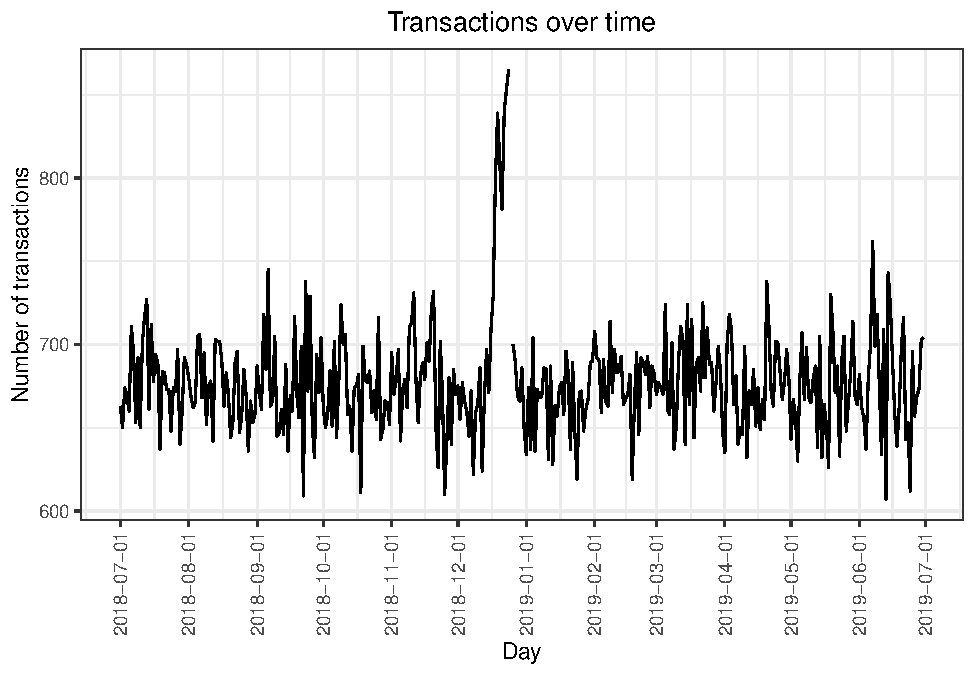
\includegraphics{quantium_analysis_files/figure-latex/unnamed-chunk-17-1} \end{center}

There is an increase in purchases in December and a break in late
December.

\hypertarget{filter-to-december-and-look-at-individual-days}{%
\paragraph{Filter to December and look at individual
days}\label{filter-to-december-and-look-at-individual-days}}

\begin{Shaded}
\begin{Highlighting}[]
\NormalTok{december\_data }\OtherTok{\textless{}{-}} \FunctionTok{subset}\NormalTok{(transaction\_by\_day, }\FunctionTok{format}\NormalTok{(date, }\StringTok{"\%m"}\NormalTok{) }\SpecialCharTok{==} \StringTok{"12"}\NormalTok{)}

\FunctionTok{ggplot}\NormalTok{(december\_data, }\FunctionTok{aes}\NormalTok{(}\AttributeTok{x =}\NormalTok{ date, }\AttributeTok{y =}\NormalTok{ N)) }\SpecialCharTok{+}
\FunctionTok{geom\_line}\NormalTok{() }\SpecialCharTok{+}
\FunctionTok{labs}\NormalTok{(}\AttributeTok{x =} \StringTok{"Day"}\NormalTok{, }\AttributeTok{y =} \StringTok{"Number of transactions"}\NormalTok{, }\AttributeTok{title =} \StringTok{"Transactions over time"}\NormalTok{) }\SpecialCharTok{+}
\FunctionTok{scale\_x\_date}\NormalTok{(}\AttributeTok{breaks =} \StringTok{"1 day"}\NormalTok{) }\SpecialCharTok{+}  \FunctionTok{theme}\NormalTok{(}\AttributeTok{axis.text.x =} \FunctionTok{element\_text}\NormalTok{(}\AttributeTok{angle =} \DecValTok{90}\NormalTok{, }\AttributeTok{vjust =} \FloatTok{0.5}\NormalTok{))}
\end{Highlighting}
\end{Shaded}

\begin{center}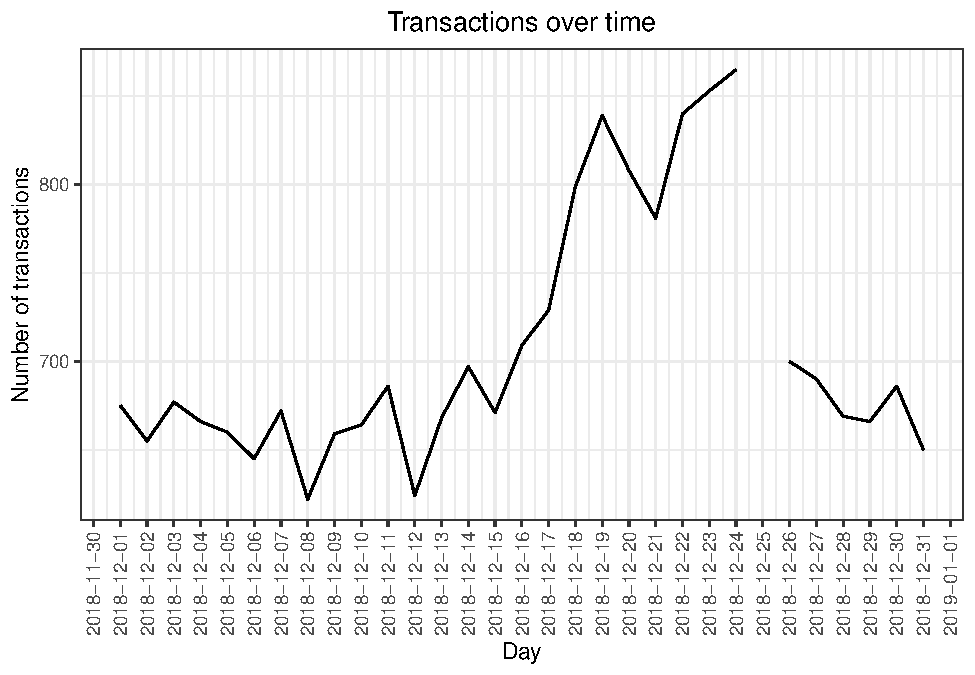
\includegraphics{quantium_analysis_files/figure-latex/unnamed-chunk-18-1} \end{center}

We can see that the increase in sales occurs in the lead-up to Christmas
and that there are zero sales on Christmas day itself. This is due to
shops being closed on Christmas day.

Now that we are satisfied that the data no longer has outliers, we can
move on to creating other features such as brand of chips or pack size
from PROD\_NAME. We will start with pack size. \#\#\#\# Pack size We can
work this out by taking the digits that are in prod\_name

\begin{Shaded}
\begin{Highlighting}[]
\NormalTok{new\_transaction\_dt[, pack\_size }\SpecialCharTok{:=} \FunctionTok{parse\_number}\NormalTok{(prod\_name)]}
\NormalTok{new\_transaction\_dt}
\end{Highlighting}
\end{Shaded}

\begin{verbatim}
##               date store_nbr lylty_card_nbr txn_id prod_nbr
##      1: 2018-10-17         1           1000      1        5
##      2: 2019-05-14         1           1307    348       66
##      3: 2019-05-20         1           1343    383       61
##      4: 2018-08-17         2           2373    974       69
##      5: 2018-08-18         2           2426   1038      108
##     ---                                                    
## 246736: 2019-03-09       272         272319 270088       89
## 246737: 2018-08-13       272         272358 270154       74
## 246738: 2018-11-06       272         272379 270187       51
## 246739: 2018-12-27       272         272379 270188       42
## 246740: 2018-09-22       272         272380 270189       74
##                                        prod_name prod_qty tot_sales pack_size
##      1:   Natural Chip        Compny SeaSalt175g        2       6.0       175
##      2:                 CCs Nacho Cheese    175g        3       6.3       175
##      3:   Smiths Crinkle Cut  Chips Chicken 170g        2       2.9       170
##      4:   Smiths Chip Thinly  S/Cream&Onion 175g        5      15.0       175
##      5: Kettle Tortilla ChpsHny&Jlpno Chili 150g        3      13.8       150
##     ---                                                                      
## 246736:  Kettle Sweet Chilli And Sour Cream 175g        2      10.8       175
## 246737:            Tostitos Splash Of  Lime 175g        1       4.4       175
## 246738:                 Doritos Mexicana    170g        2       8.8       170
## 246739:  Doritos Corn Chip Mexican Jalapeno 150g        2       7.8       150
## 246740:            Tostitos Splash Of  Lime 175g        2       8.8       175
\end{verbatim}

\hypertarget{check-if-the-pack-sizes-look-sensible}{%
\paragraph{Check if the pack sizes look
sensible}\label{check-if-the-pack-sizes-look-sensible}}

\begin{Shaded}
\begin{Highlighting}[]
\NormalTok{transaction\_pack\_size }\OtherTok{\textless{}{-}}\NormalTok{ new\_transaction\_dt[, .N,pack\_size][}\FunctionTok{order}\NormalTok{(pack\_size)]}
\NormalTok{transaction\_pack\_size}
\end{Highlighting}
\end{Shaded}

\begin{verbatim}
##     pack_size     N
##  1:        70  1507
##  2:        90  3008
##  3:       110 22387
##  4:       125  1454
##  5:       134 25102
##  6:       135  3257
##  7:       150 40203
##  8:       160  2970
##  9:       165 15297
## 10:       170 19983
## 11:       175 66390
## 12:       180  1468
## 13:       190  2995
## 14:       200  4473
## 15:       210  6272
## 16:       220  1564
## 17:       250  3169
## 18:       270  6285
## 19:       330 12540
## 20:       380  6416
\end{verbatim}

The largest size is 380g and the smallest size is 70g - seems sensible!

\hypertarget{plot-a-histogram-showing-the-number-of-transactions-by-pack-size}{%
\paragraph{Plot a histogram showing the number of transactions by pack
size}\label{plot-a-histogram-showing-the-number-of-transactions-by-pack-size}}

\begin{Shaded}
\begin{Highlighting}[]
\FunctionTok{hist}\NormalTok{(transaction\_pack\_size[,pack\_size])}
\end{Highlighting}
\end{Shaded}

\begin{center}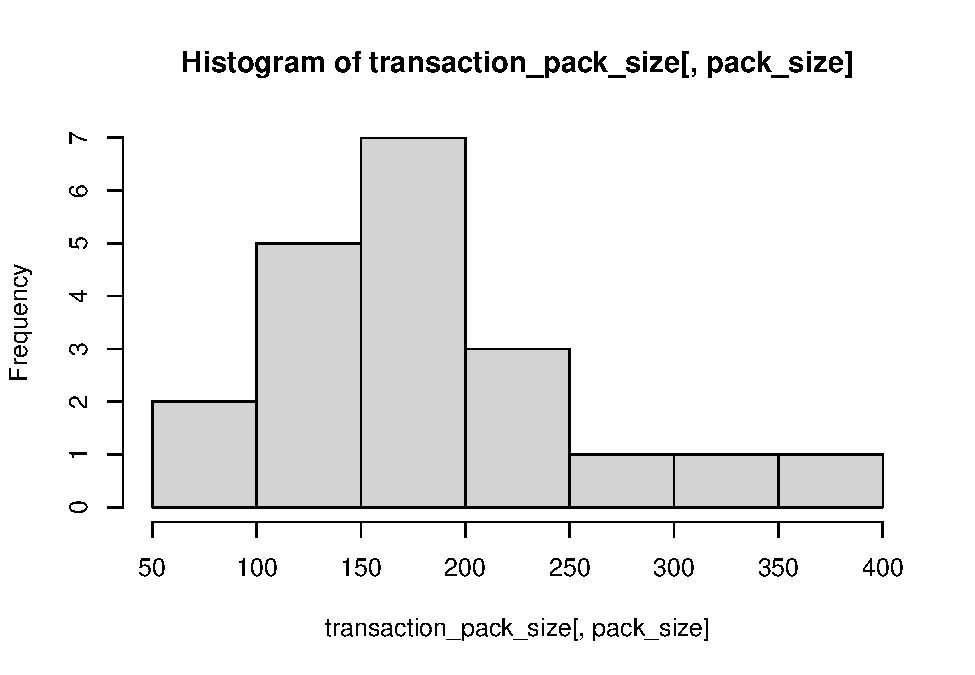
\includegraphics{quantium_analysis_files/figure-latex/unnamed-chunk-21-1} \end{center}

\hypertarget{create-brands}{%
\paragraph{Create brands}\label{create-brands}}

Create a column which contains the brand of the product, by extracting
it from the product name

\begin{Shaded}
\begin{Highlighting}[]
\NormalTok{brand\_transaction }\OtherTok{\textless{}{-}}\NormalTok{ new\_transaction\_dt }\SpecialCharTok{\%\textgreater{}\%}
  \FunctionTok{mutate}\NormalTok{(}\AttributeTok{brand =} \FunctionTok{toupper}\NormalTok{ (}\FunctionTok{str\_extract}\NormalTok{(prod\_name, }\StringTok{"[a{-}zA{-}Z]+"}\NormalTok{)))}
\NormalTok{brand\_transaction}\SpecialCharTok{\%\textgreater{}\%} \FunctionTok{select}\NormalTok{(brand)}\SpecialCharTok{\%\textgreater{}\%}\FunctionTok{group\_by}\NormalTok{(brand)}
\end{Highlighting}
\end{Shaded}

\begin{verbatim}
## # A tibble: 246,740 x 1
## # Groups:   brand [28]
##    brand  
##    <chr>  
##  1 NATURAL
##  2 CCS    
##  3 SMITHS 
##  4 SMITHS 
##  5 KETTLE 
##  6 SMITHS 
##  7 GRAIN  
##  8 DORITOS
##  9 GRAIN  
## 10 SMITHS 
## # i 246,730 more rows
\end{verbatim}

Some of the brand names look like they are of the same brands - such as
RED and RRD, which are both Red Rock Deli chips

\hypertarget{clean-brand-names}{%
\paragraph{Clean brand names}\label{clean-brand-names}}

\begin{Shaded}
\begin{Highlighting}[]
\NormalTok{brand\_transaction[brand}\SpecialCharTok{==} \StringTok{"RED"}\NormalTok{,brand }\SpecialCharTok{:=} \StringTok{"RRD"}\NormalTok{] }
\NormalTok{brand\_transaction[brand}\SpecialCharTok{==} \StringTok{"SNBTS"}\NormalTok{,brand }\SpecialCharTok{:=} \StringTok{"SUNBITES"}\NormalTok{] }
\NormalTok{brand\_transaction[brand}\SpecialCharTok{==} \StringTok{"INFZNS"}\NormalTok{,brand }\SpecialCharTok{:=} \StringTok{"INFUZIONS"}\NormalTok{] }
\NormalTok{brand\_transaction[brand}\SpecialCharTok{==} \StringTok{"WW"}\NormalTok{,brand }\SpecialCharTok{:=} \StringTok{"WOOLWORTHS"}\NormalTok{] }
\NormalTok{brand\_transaction[brand}\SpecialCharTok{==} \StringTok{"SMITH"}\NormalTok{,brand }\SpecialCharTok{:=} \StringTok{"SMITHS"}\NormalTok{] }
\NormalTok{brand\_transaction[brand}\SpecialCharTok{==} \StringTok{"NCC"}\NormalTok{,brand }\SpecialCharTok{:=} \StringTok{"NATURAL"}\NormalTok{] }
\NormalTok{brand\_transaction[brand}\SpecialCharTok{==} \StringTok{"DORITO"}\NormalTok{,brand }\SpecialCharTok{:=} \StringTok{"DORITOS"}\NormalTok{] }
\NormalTok{brand\_transaction[brand}\SpecialCharTok{==} \StringTok{"GRAIN"}\NormalTok{,brand }\SpecialCharTok{:=} \StringTok{"GRNWVES"}\NormalTok{]}
\NormalTok{fix\_transaction }\OtherTok{\textless{}{-}}\NormalTok{ brand\_transaction}
\NormalTok{fix\_transaction}
\end{Highlighting}
\end{Shaded}

\begin{verbatim}
##               date store_nbr lylty_card_nbr txn_id prod_nbr
##      1: 2018-10-17         1           1000      1        5
##      2: 2019-05-14         1           1307    348       66
##      3: 2019-05-20         1           1343    383       61
##      4: 2018-08-17         2           2373    974       69
##      5: 2018-08-18         2           2426   1038      108
##     ---                                                    
## 246736: 2019-03-09       272         272319 270088       89
## 246737: 2018-08-13       272         272358 270154       74
## 246738: 2018-11-06       272         272379 270187       51
## 246739: 2018-12-27       272         272379 270188       42
## 246740: 2018-09-22       272         272380 270189       74
##                                        prod_name prod_qty tot_sales pack_size
##      1:   Natural Chip        Compny SeaSalt175g        2       6.0       175
##      2:                 CCs Nacho Cheese    175g        3       6.3       175
##      3:   Smiths Crinkle Cut  Chips Chicken 170g        2       2.9       170
##      4:   Smiths Chip Thinly  S/Cream&Onion 175g        5      15.0       175
##      5: Kettle Tortilla ChpsHny&Jlpno Chili 150g        3      13.8       150
##     ---                                                                      
## 246736:  Kettle Sweet Chilli And Sour Cream 175g        2      10.8       175
## 246737:            Tostitos Splash Of  Lime 175g        1       4.4       175
## 246738:                 Doritos Mexicana    170g        2       8.8       170
## 246739:  Doritos Corn Chip Mexican Jalapeno 150g        2       7.8       150
## 246740:            Tostitos Splash Of  Lime 175g        2       8.8       175
##            brand
##      1:  NATURAL
##      2:      CCS
##      3:   SMITHS
##      4:   SMITHS
##      5:   KETTLE
##     ---         
## 246736:   KETTLE
## 246737: TOSTITOS
## 246738:  DORITOS
## 246739:  DORITOS
## 246740: TOSTITOS
\end{verbatim}

\hypertarget{examining-customer-data}{%
\subsection{Examining Customer Data}\label{examining-customer-data}}

\begin{Shaded}
\begin{Highlighting}[]
\NormalTok{purchase\_df }\OtherTok{\textless{}{-}} \FunctionTok{clean\_names}\NormalTok{(purchase\_behaviour)}
\FunctionTok{summary}\NormalTok{(purchase\_df)}
\end{Highlighting}
\end{Shaded}

\begin{verbatim}
##  lylty_card_nbr     lifestage         premium_customer  
##  Min.   :   1000   Length:72637       Length:72637      
##  1st Qu.:  66202   Class :character   Class :character  
##  Median : 134040   Mode  :character   Mode  :character  
##  Mean   : 136186                                        
##  3rd Qu.: 203375                                        
##  Max.   :2373711
\end{verbatim}

\hypertarget{merge-transaction-data-to-customer-data}{%
\paragraph{Merge transaction data to customer
data}\label{merge-transaction-data-to-customer-data}}

\begin{Shaded}
\begin{Highlighting}[]
\NormalTok{all\_data }\OtherTok{\textless{}{-}} \FunctionTok{merge}\NormalTok{(fix\_transaction, purchase\_df, }\AttributeTok{all.x =} \ConstantTok{TRUE}\NormalTok{)}
\NormalTok{all\_data}
\end{Highlighting}
\end{Shaded}

\begin{verbatim}
##         lylty_card_nbr       date store_nbr txn_id prod_nbr
##      1:           1000 2018-10-17         1      1        5
##      2:           1002 2018-09-16         1      2       58
##      3:           1003 2019-03-07         1      3       52
##      4:           1003 2019-03-08         1      4      106
##      5:           1004 2018-11-02         1      5       96
##     ---                                                    
## 246736:        2370651 2018-08-03        88 240350        4
## 246737:        2370701 2018-12-08        88 240378       24
## 246738:        2370751 2018-10-01        88 240394       60
## 246739:        2370961 2018-10-24        88 240480       70
## 246740:        2373711 2018-12-14        88 241815       16
##                                        prod_name prod_qty tot_sales pack_size
##      1:   Natural Chip        Compny SeaSalt175g        2       6.0       175
##      2:    Red Rock Deli Chikn&Garlic Aioli 150g        1       2.7       150
##      3:    Grain Waves Sour    Cream&Chives 210G        1       3.6       210
##      4:   Natural ChipCo      Hony Soy Chckn175g        1       3.0       175
##      5:           WW Original Stacked Chips 160g        1       1.9       160
##     ---                                                                      
## 246736:         Dorito Corn Chp     Supreme 380g        2      13.0       380
## 246737:    Grain Waves         Sweet Chilli 210g        2       7.2       210
## 246738:     Kettle Tortilla ChpsFeta&Garlic 150g        2       9.2       150
## 246739:  Tyrrells Crisps     Lightly Salted 165g        2       8.4       165
## 246740: Smiths Crinkle Chips Salt & Vinegar 330g        2      11.4       330
##              brand              lifestage premium_customer
##      1:    NATURAL  YOUNG SINGLES/COUPLES          Premium
##      2:        RRD  YOUNG SINGLES/COUPLES       Mainstream
##      3:    GRNWVES         YOUNG FAMILIES           Budget
##      4:    NATURAL         YOUNG FAMILIES           Budget
##      5: WOOLWORTHS  OLDER SINGLES/COUPLES       Mainstream
##     ---                                                   
## 246736:    DORITOS MIDAGE SINGLES/COUPLES       Mainstream
## 246737:    GRNWVES         YOUNG FAMILIES       Mainstream
## 246738:     KETTLE         YOUNG FAMILIES          Premium
## 246739:   TYRRELLS         OLDER FAMILIES           Budget
## 246740:     SMITHS  YOUNG SINGLES/COUPLES       Mainstream
\end{verbatim}

As the number of rows in all\_data is the same as that of
clean\_transaction, we can be sure that no duplicates were created. This
is because we created all\_data by setting all.x = TRUE (in other words,
a left join) which means take all the rows in clean\_transaction and
find rows with matching values in shared columns and then joining the
details in these rows to the x or the first mentioned table.

\hypertarget{see-if-any-transactions-did-not-have-a-matched-customer}{%
\paragraph{See if any transactions did not have a matched
customer}\label{see-if-any-transactions-did-not-have-a-matched-customer}}

\begin{Shaded}
\begin{Highlighting}[]
\FunctionTok{skim\_without\_charts}\NormalTok{(all\_data)}
\end{Highlighting}
\end{Shaded}

\begin{longtable}[]{@{}ll@{}}
\caption{Data summary}\tabularnewline
\toprule\noalign{}
\endfirsthead
\endhead
\bottomrule\noalign{}
\endlastfoot
Name & all\_data \\
Number of rows & 246740 \\
Number of columns & 12 \\
Key & lylty\_card\_nbr \\
\_\_\_\_\_\_\_\_\_\_\_\_\_\_\_\_\_\_\_\_\_\_\_ & \\
Column type frequency: & \\
character & 4 \\
Date & 1 \\
numeric & 7 \\
\_\_\_\_\_\_\_\_\_\_\_\_\_\_\_\_\_\_\_\_\_\_\_\_ & \\
Group variables & None \\
\end{longtable}

\textbf{Variable type: character}

\begin{longtable}[]{@{}
  >{\raggedright\arraybackslash}p{(\columnwidth - 14\tabcolsep) * \real{0.2267}}
  >{\raggedleft\arraybackslash}p{(\columnwidth - 14\tabcolsep) * \real{0.1333}}
  >{\raggedleft\arraybackslash}p{(\columnwidth - 14\tabcolsep) * \real{0.1867}}
  >{\raggedleft\arraybackslash}p{(\columnwidth - 14\tabcolsep) * \real{0.0533}}
  >{\raggedleft\arraybackslash}p{(\columnwidth - 14\tabcolsep) * \real{0.0533}}
  >{\raggedleft\arraybackslash}p{(\columnwidth - 14\tabcolsep) * \real{0.0800}}
  >{\raggedleft\arraybackslash}p{(\columnwidth - 14\tabcolsep) * \real{0.1200}}
  >{\raggedleft\arraybackslash}p{(\columnwidth - 14\tabcolsep) * \real{0.1467}}@{}}
\toprule\noalign{}
\begin{minipage}[b]{\linewidth}\raggedright
skim\_variable
\end{minipage} & \begin{minipage}[b]{\linewidth}\raggedleft
n\_missing
\end{minipage} & \begin{minipage}[b]{\linewidth}\raggedleft
complete\_rate
\end{minipage} & \begin{minipage}[b]{\linewidth}\raggedleft
min
\end{minipage} & \begin{minipage}[b]{\linewidth}\raggedleft
max
\end{minipage} & \begin{minipage}[b]{\linewidth}\raggedleft
empty
\end{minipage} & \begin{minipage}[b]{\linewidth}\raggedleft
n\_unique
\end{minipage} & \begin{minipage}[b]{\linewidth}\raggedleft
whitespace
\end{minipage} \\
\midrule\noalign{}
\endhead
\bottomrule\noalign{}
\endlastfoot
prod\_name & 0 & 1 & 17 & 40 & 0 & 105 & 0 \\
brand & 0 & 1 & 3 & 10 & 0 & 20 & 0 \\
lifestage & 0 & 1 & 8 & 22 & 0 & 7 & 0 \\
premium\_customer & 0 & 1 & 6 & 10 & 0 & 3 & 0 \\
\end{longtable}

\textbf{Variable type: Date}

\begin{longtable}[]{@{}
  >{\raggedright\arraybackslash}p{(\columnwidth - 12\tabcolsep) * \real{0.1750}}
  >{\raggedleft\arraybackslash}p{(\columnwidth - 12\tabcolsep) * \real{0.1250}}
  >{\raggedleft\arraybackslash}p{(\columnwidth - 12\tabcolsep) * \real{0.1750}}
  >{\raggedright\arraybackslash}p{(\columnwidth - 12\tabcolsep) * \real{0.1375}}
  >{\raggedright\arraybackslash}p{(\columnwidth - 12\tabcolsep) * \real{0.1375}}
  >{\raggedright\arraybackslash}p{(\columnwidth - 12\tabcolsep) * \real{0.1375}}
  >{\raggedleft\arraybackslash}p{(\columnwidth - 12\tabcolsep) * \real{0.1125}}@{}}
\toprule\noalign{}
\begin{minipage}[b]{\linewidth}\raggedright
skim\_variable
\end{minipage} & \begin{minipage}[b]{\linewidth}\raggedleft
n\_missing
\end{minipage} & \begin{minipage}[b]{\linewidth}\raggedleft
complete\_rate
\end{minipage} & \begin{minipage}[b]{\linewidth}\raggedright
min
\end{minipage} & \begin{minipage}[b]{\linewidth}\raggedright
max
\end{minipage} & \begin{minipage}[b]{\linewidth}\raggedright
median
\end{minipage} & \begin{minipage}[b]{\linewidth}\raggedleft
n\_unique
\end{minipage} \\
\midrule\noalign{}
\endhead
\bottomrule\noalign{}
\endlastfoot
date & 0 & 1 & 2018-07-01 & 2019-06-30 & 2018-12-30 & 364 \\
\end{longtable}

\textbf{Variable type: numeric}

\begin{longtable}[]{@{}
  >{\raggedright\arraybackslash}p{(\columnwidth - 18\tabcolsep) * \real{0.1471}}
  >{\raggedleft\arraybackslash}p{(\columnwidth - 18\tabcolsep) * \real{0.0980}}
  >{\raggedleft\arraybackslash}p{(\columnwidth - 18\tabcolsep) * \real{0.1373}}
  >{\raggedleft\arraybackslash}p{(\columnwidth - 18\tabcolsep) * \real{0.0980}}
  >{\raggedleft\arraybackslash}p{(\columnwidth - 18\tabcolsep) * \real{0.0882}}
  >{\raggedleft\arraybackslash}p{(\columnwidth - 18\tabcolsep) * \real{0.0686}}
  >{\raggedleft\arraybackslash}p{(\columnwidth - 18\tabcolsep) * \real{0.0882}}
  >{\raggedleft\arraybackslash}p{(\columnwidth - 18\tabcolsep) * \real{0.0882}}
  >{\raggedleft\arraybackslash}p{(\columnwidth - 18\tabcolsep) * \real{0.0882}}
  >{\raggedleft\arraybackslash}p{(\columnwidth - 18\tabcolsep) * \real{0.0980}}@{}}
\toprule\noalign{}
\begin{minipage}[b]{\linewidth}\raggedright
skim\_variable
\end{minipage} & \begin{minipage}[b]{\linewidth}\raggedleft
n\_missing
\end{minipage} & \begin{minipage}[b]{\linewidth}\raggedleft
complete\_rate
\end{minipage} & \begin{minipage}[b]{\linewidth}\raggedleft
mean
\end{minipage} & \begin{minipage}[b]{\linewidth}\raggedleft
sd
\end{minipage} & \begin{minipage}[b]{\linewidth}\raggedleft
p0
\end{minipage} & \begin{minipage}[b]{\linewidth}\raggedleft
p25
\end{minipage} & \begin{minipage}[b]{\linewidth}\raggedleft
p50
\end{minipage} & \begin{minipage}[b]{\linewidth}\raggedleft
p75
\end{minipage} & \begin{minipage}[b]{\linewidth}\raggedleft
p100
\end{minipage} \\
\midrule\noalign{}
\endhead
\bottomrule\noalign{}
\endlastfoot
lylty\_card\_nbr & 0 & 1 & 135530.25 & 80715.20 & 1000.0 & 70015.00 &
130367.0 & 203083.2 & 2373711.0 \\
store\_nbr & 0 & 1 & 135.05 & 76.79 & 1.0 & 70.00 & 130.0 & 203.0 &
272.0 \\
txn\_id & 0 & 1 & 135130.36 & 78147.60 & 1.0 & 67568.75 & 135181.5 &
202652.2 & 2415841.0 \\
prod\_nbr & 0 & 1 & 56.35 & 33.70 & 1.0 & 26.00 & 53.0 & 87.0 & 114.0 \\
prod\_qty & 0 & 1 & 1.91 & 0.34 & 1.0 & 2.00 & 2.0 & 2.0 & 5.0 \\
tot\_sales & 0 & 1 & 7.32 & 2.47 & 1.7 & 5.80 & 7.4 & 8.8 & 29.5 \\
pack\_size & 0 & 1 & 175.58 & 59.43 & 70.0 & 150.00 & 170.0 & 175.0 &
380.0 \\
\end{longtable}

There are no nulls. So all our customers in the transaction data has
been accounted for in the customer dataset

\begin{Shaded}
\begin{Highlighting}[]
\FunctionTok{write.csv}\NormalTok{(all\_data, }\StringTok{"all\_data.csv"}\NormalTok{,}\AttributeTok{row.names =} \ConstantTok{FALSE}\NormalTok{)}
\end{Highlighting}
\end{Shaded}

\hypertarget{data-exploration-is-now-complete}{%
\paragraph{Data exploration is now
complete}\label{data-exploration-is-now-complete}}

\hypertarget{data-analysis-in-customer-segments}{%
\subsection{Data Analysis in Customer
Segments}\label{data-analysis-in-customer-segments}}

Now that the data is ready for analysis, we can define some metrics of
interest to the client: * Who spends the most on chips (total sales),
describing customers by lifestage and how premium their general
purchasing behaviour is * How many customers are in each segment * How
many chips are bought per customer by segment * What's the average chip
price by customer segment

We could also ask our data team for more information. Examples are: *
The customer's total spend over the period and total spend for each
transaction to understand what proportion of their grocery spend is on
chips * Proportion of customers in each customer segment overall to
compare against the mix of customers who purchase chips

Let's start with calculating total sales by LIFESTAGE and
PREMIUM\_CUSTOMER and plotting the split by these segments to describe
which customer segment contribute most to chip sales. \#\#\#\# Total
sales by lifestage and premium\_customer

\begin{Shaded}
\begin{Highlighting}[]
\NormalTok{all\_data }\SpecialCharTok{\%\textgreater{}\%}
  \FunctionTok{group\_by}\NormalTok{(lifestage, premium\_customer) }\SpecialCharTok{\%\textgreater{}\%}
  \FunctionTok{summarize}\NormalTok{(}\AttributeTok{total\_sales =} \FunctionTok{sum}\NormalTok{(tot\_sales)) }\SpecialCharTok{\%\textgreater{}\%}
  \FunctionTok{arrange}\NormalTok{(}\FunctionTok{desc}\NormalTok{(total\_sales))}
\end{Highlighting}
\end{Shaded}

\begin{verbatim}
## `summarise()` has grouped output by 'lifestage'. You can override using the
## `.groups` argument.
\end{verbatim}

\begin{verbatim}
## # A tibble: 21 x 3
## # Groups:   lifestage [7]
##    lifestage             premium_customer total_sales
##    <chr>                 <chr>                  <dbl>
##  1 OLDER FAMILIES        Budget               156864.
##  2 YOUNG SINGLES/COUPLES Mainstream           147582.
##  3 RETIREES              Mainstream           145169.
##  4 YOUNG FAMILIES        Budget               129718.
##  5 OLDER SINGLES/COUPLES Budget               127834.
##  6 OLDER SINGLES/COUPLES Mainstream           124648.
##  7 OLDER SINGLES/COUPLES Premium              123538.
##  8 RETIREES              Budget               105916.
##  9 OLDER FAMILIES        Mainstream            96414.
## 10 RETIREES              Premium               91297.
## # i 11 more rows
\end{verbatim}

\hypertarget{create-a-plot}{%
\paragraph{Create a plot}\label{create-a-plot}}

\begin{Shaded}
\begin{Highlighting}[]
\NormalTok{total\_sales\_by\_segment }\OtherTok{\textless{}{-}}\NormalTok{ all\_data }\SpecialCharTok{\%\textgreater{}\%}
  \FunctionTok{group\_by}\NormalTok{(lifestage, premium\_customer) }\SpecialCharTok{\%\textgreater{}\%}
  \FunctionTok{summarize}\NormalTok{(}\AttributeTok{total\_sales =} \FunctionTok{sum}\NormalTok{(tot\_sales))}
\end{Highlighting}
\end{Shaded}

\begin{verbatim}
## `summarise()` has grouped output by 'lifestage'. You can override using the
## `.groups` argument.
\end{verbatim}

\begin{Shaded}
\begin{Highlighting}[]
\CommentTok{\# Plotting the results}
\FunctionTok{ggplot}\NormalTok{(total\_sales\_by\_segment, }\FunctionTok{aes}\NormalTok{(}\AttributeTok{x =}\NormalTok{ lifestage, }\AttributeTok{y =}\NormalTok{ total\_sales, }\AttributeTok{fill =}\NormalTok{ premium\_customer)) }\SpecialCharTok{+}
  \FunctionTok{geom\_bar}\NormalTok{(}\AttributeTok{stat =} \StringTok{"identity"}\NormalTok{, }\AttributeTok{position =} \StringTok{"dodge"}\NormalTok{) }\SpecialCharTok{+}
  \FunctionTok{labs}\NormalTok{(}\AttributeTok{title =} \StringTok{"Total Sales by Lifestage and Premium Customer"}\NormalTok{,}
       \AttributeTok{x =} \StringTok{"Lifestage"}\NormalTok{,}
       \AttributeTok{y =} \StringTok{"Total Sales"}\NormalTok{) }\SpecialCharTok{+}
  \FunctionTok{theme}\NormalTok{(}\AttributeTok{axis.text.x=} \FunctionTok{element\_text}\NormalTok{(}\AttributeTok{angle=}\DecValTok{90}\NormalTok{,}\AttributeTok{vjust=}\FloatTok{0.5}\NormalTok{))}\SpecialCharTok{+}
  \FunctionTok{scale\_fill\_brewer}\NormalTok{(}\AttributeTok{palette =} \StringTok{"Paired"}\NormalTok{)}
\end{Highlighting}
\end{Shaded}

\begin{center}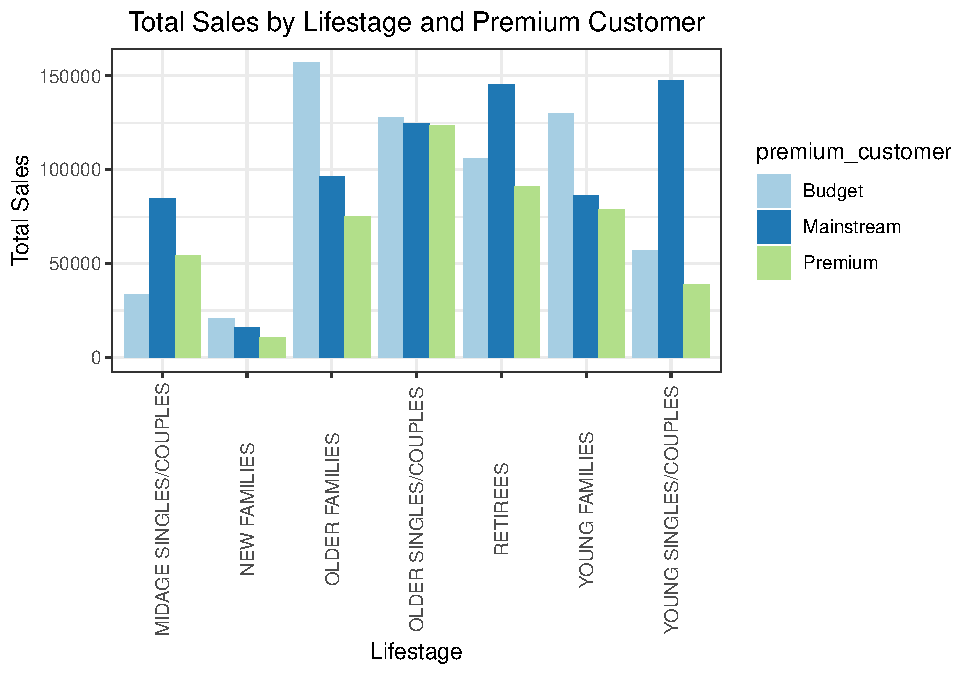
\includegraphics{quantium_analysis_files/figure-latex/unnamed-chunk-29-1} \end{center}

Sales are coming mainly from * Budget - older families, * Mainstream -
young singles/couples, and * Mainstream - retirees

\hypertarget{number-of-customers-by-lifestage-and-premium_customer}{%
\paragraph{Number of customers by lifestage and
premium\_customer}\label{number-of-customers-by-lifestage-and-premium_customer}}

\begin{Shaded}
\begin{Highlighting}[]
\NormalTok{all\_data }\SpecialCharTok{\%\textgreater{}\%}
  \FunctionTok{group\_by}\NormalTok{(lifestage, premium\_customer) }\SpecialCharTok{\%\textgreater{}\%}
  \FunctionTok{summarize}\NormalTok{(}\AttributeTok{total\_customer =} \FunctionTok{n\_distinct}\NormalTok{(lylty\_card\_nbr),}
            \AttributeTok{total\_customer =} \FunctionTok{sum}\NormalTok{(lylty\_card\_nbr)) }\SpecialCharTok{\%\textgreater{}\%}
  \FunctionTok{arrange}\NormalTok{(}\FunctionTok{desc}\NormalTok{(total\_customer))}
\end{Highlighting}
\end{Shaded}

\begin{verbatim}
## `summarise()` has grouped output by 'lifestage'. You can override using the
## `.groups` argument.
\end{verbatim}

\begin{verbatim}
## # A tibble: 21 x 3
## # Groups:   lifestage [7]
##    lifestage             premium_customer total_customer
##    <chr>                 <chr>                     <dbl>
##  1 OLDER FAMILIES        Budget               2891942530
##  2 RETIREES              Mainstream           2753153856
##  3 YOUNG SINGLES/COUPLES Mainstream           2637061979
##  4 YOUNG FAMILIES        Budget               2415761554
##  5 OLDER SINGLES/COUPLES Budget               2332495098
##  6 OLDER SINGLES/COUPLES Mainstream           2279764274
##  7 OLDER SINGLES/COUPLES Premium              2228223157
##  8 RETIREES              Budget               1927702126
##  9 OLDER FAMILIES        Mainstream           1782766792
## 10 RETIREES              Premium              1660094379
## # i 11 more rows
\end{verbatim}

\hypertarget{create-a-plot-1}{%
\paragraph{Create a plot}\label{create-a-plot-1}}

\begin{Shaded}
\begin{Highlighting}[]
\NormalTok{total\_customer\_by\_segment }\OtherTok{\textless{}{-}}\NormalTok{ all\_data }\SpecialCharTok{\%\textgreater{}\%}
  \FunctionTok{group\_by}\NormalTok{(lifestage, premium\_customer) }\SpecialCharTok{\%\textgreater{}\%}
  \FunctionTok{summarize}\NormalTok{(}\AttributeTok{total\_customer =} \FunctionTok{n\_distinct}\NormalTok{(lylty\_card\_nbr),}
            \AttributeTok{total\_customer =} \FunctionTok{sum}\NormalTok{(lylty\_card\_nbr)) }\SpecialCharTok{\%\textgreater{}\%}
  \FunctionTok{arrange}\NormalTok{(}\FunctionTok{desc}\NormalTok{(total\_customer))}
\end{Highlighting}
\end{Shaded}

\begin{verbatim}
## `summarise()` has grouped output by 'lifestage'. You can override using the
## `.groups` argument.
\end{verbatim}

\begin{Shaded}
\begin{Highlighting}[]
\CommentTok{\# Plotting the results}
\FunctionTok{ggplot}\NormalTok{(total\_customer\_by\_segment, }\FunctionTok{aes}\NormalTok{(}\AttributeTok{x =}\NormalTok{ lifestage, }\AttributeTok{y =}\NormalTok{ total\_customer, }\AttributeTok{fill =}\NormalTok{ premium\_customer)) }\SpecialCharTok{+}
  \FunctionTok{geom\_bar}\NormalTok{(}\AttributeTok{stat =} \StringTok{"identity"}\NormalTok{, }\AttributeTok{position =} \StringTok{"dodge"}\NormalTok{) }\SpecialCharTok{+}
  \FunctionTok{labs}\NormalTok{(}\AttributeTok{title =} \StringTok{"Total Customer by Lifestage and Premium Customer"}\NormalTok{,}
       \AttributeTok{x =} \StringTok{"Lifestage"}\NormalTok{,}
       \AttributeTok{y =} \StringTok{"Total Customer"}\NormalTok{) }\SpecialCharTok{+}
  \FunctionTok{theme}\NormalTok{(}\AttributeTok{axis.text.x=} \FunctionTok{element\_text}\NormalTok{(}\AttributeTok{angle=}\DecValTok{90}\NormalTok{,}\AttributeTok{vjust=}\FloatTok{0.5}\NormalTok{))}\SpecialCharTok{+}
  \FunctionTok{scale\_fill\_brewer}\NormalTok{(}\AttributeTok{palette =} \StringTok{"Paired"}\NormalTok{)}
\end{Highlighting}
\end{Shaded}

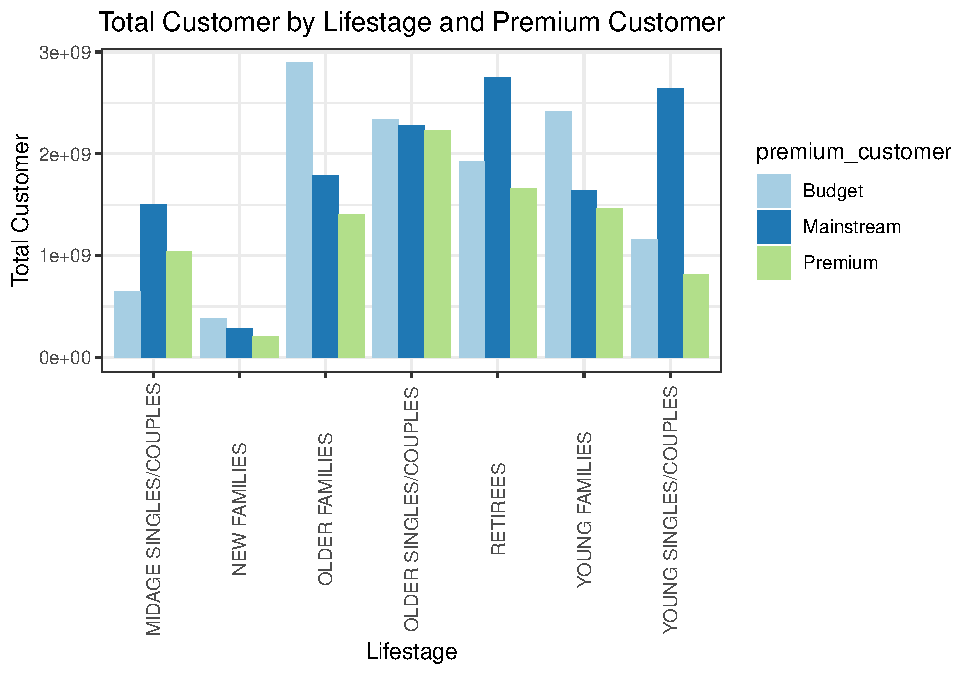
\includegraphics{quantium_analysis_files/figure-latex/unnamed-chunk-31-1.pdf}
There are more Mainstream - young singles/couples and Mainstream -
retirees who buy chips. This contributes to there being more sales to
these customer segments but this is not a major driver for the Budget -
Older families segment.

Higher sales may also be driven by more units of chips being bought per
customer.

\hypertarget{average-number-of-units-per-customer-by-lifestage-and-premium_customer}{%
\paragraph{Average number of units per customer by lifestage and
premium\_customer}\label{average-number-of-units-per-customer-by-lifestage-and-premium_customer}}

\begin{Shaded}
\begin{Highlighting}[]
\NormalTok{all\_data }\SpecialCharTok{\%\textgreater{}\%}
  \FunctionTok{group\_by}\NormalTok{(lifestage, premium\_customer) }\SpecialCharTok{\%\textgreater{}\%}
  \FunctionTok{summarize}\NormalTok{(}\AttributeTok{avg\_unit =} \FunctionTok{sum}\NormalTok{(prod\_qty)}\SpecialCharTok{/}\FunctionTok{n\_distinct}\NormalTok{(lylty\_card\_nbr) ) }\SpecialCharTok{\%\textgreater{}\%}
  \FunctionTok{arrange}\NormalTok{(}\FunctionTok{desc}\NormalTok{(avg\_unit))}
\end{Highlighting}
\end{Shaded}

\begin{verbatim}
## `summarise()` has grouped output by 'lifestage'. You can override using the
## `.groups` argument.
\end{verbatim}

\begin{verbatim}
## # A tibble: 21 x 3
## # Groups:   lifestage [7]
##    lifestage              premium_customer avg_unit
##    <chr>                  <chr>               <dbl>
##  1 OLDER FAMILIES         Mainstream           9.26
##  2 OLDER FAMILIES         Budget               9.08
##  3 OLDER FAMILIES         Premium              9.07
##  4 YOUNG FAMILIES         Budget               8.72
##  5 YOUNG FAMILIES         Premium              8.72
##  6 YOUNG FAMILIES         Mainstream           8.64
##  7 OLDER SINGLES/COUPLES  Budget               6.78
##  8 OLDER SINGLES/COUPLES  Premium              6.77
##  9 OLDER SINGLES/COUPLES  Mainstream           6.71
## 10 MIDAGE SINGLES/COUPLES Mainstream           6.43
## # i 11 more rows
\end{verbatim}

\hypertarget{create-a-plot-2}{%
\paragraph{Create a plot}\label{create-a-plot-2}}

\begin{Shaded}
\begin{Highlighting}[]
\NormalTok{avg\_unit\_by\_segment }\OtherTok{\textless{}{-}}\NormalTok{ all\_data }\SpecialCharTok{\%\textgreater{}\%}
  \FunctionTok{group\_by}\NormalTok{(lifestage, premium\_customer) }\SpecialCharTok{\%\textgreater{}\%}
  \FunctionTok{summarize}\NormalTok{(}\AttributeTok{avg\_unit =} \FunctionTok{sum}\NormalTok{(prod\_qty)}\SpecialCharTok{/}\FunctionTok{n\_distinct}\NormalTok{(lylty\_card\_nbr) ) }\SpecialCharTok{\%\textgreater{}\%}
  \FunctionTok{arrange}\NormalTok{(}\FunctionTok{desc}\NormalTok{(avg\_unit))}
\end{Highlighting}
\end{Shaded}

\begin{verbatim}
## `summarise()` has grouped output by 'lifestage'. You can override using the
## `.groups` argument.
\end{verbatim}

\begin{Shaded}
\begin{Highlighting}[]
\CommentTok{\# Plotting the results}
\FunctionTok{ggplot}\NormalTok{(avg\_unit\_by\_segment, }\FunctionTok{aes}\NormalTok{(}\AttributeTok{x =}\NormalTok{ lifestage, }\AttributeTok{y =}\NormalTok{ avg\_unit, }\AttributeTok{fill =}\NormalTok{ premium\_customer)) }\SpecialCharTok{+}
  \FunctionTok{geom\_bar}\NormalTok{(}\AttributeTok{stat =} \StringTok{"identity"}\NormalTok{, }\AttributeTok{position =} \StringTok{"dodge"}\NormalTok{) }\SpecialCharTok{+}
  \FunctionTok{labs}\NormalTok{(}\AttributeTok{title =} \StringTok{"Units per Customer"}\NormalTok{,}
       \AttributeTok{x =} \StringTok{"Lifestage"}\NormalTok{,}
       \AttributeTok{y =} \StringTok{"Avg unit per transaction"}\NormalTok{) }\SpecialCharTok{+}
  \FunctionTok{theme}\NormalTok{(}\AttributeTok{axis.text.x=} \FunctionTok{element\_text}\NormalTok{(}\AttributeTok{angle=}\DecValTok{90}\NormalTok{,}\AttributeTok{vjust=}\FloatTok{0.5}\NormalTok{))}\SpecialCharTok{+}
  \FunctionTok{scale\_fill\_brewer}\NormalTok{(}\AttributeTok{palette =} \StringTok{"Paired"}\NormalTok{)}
\end{Highlighting}
\end{Shaded}

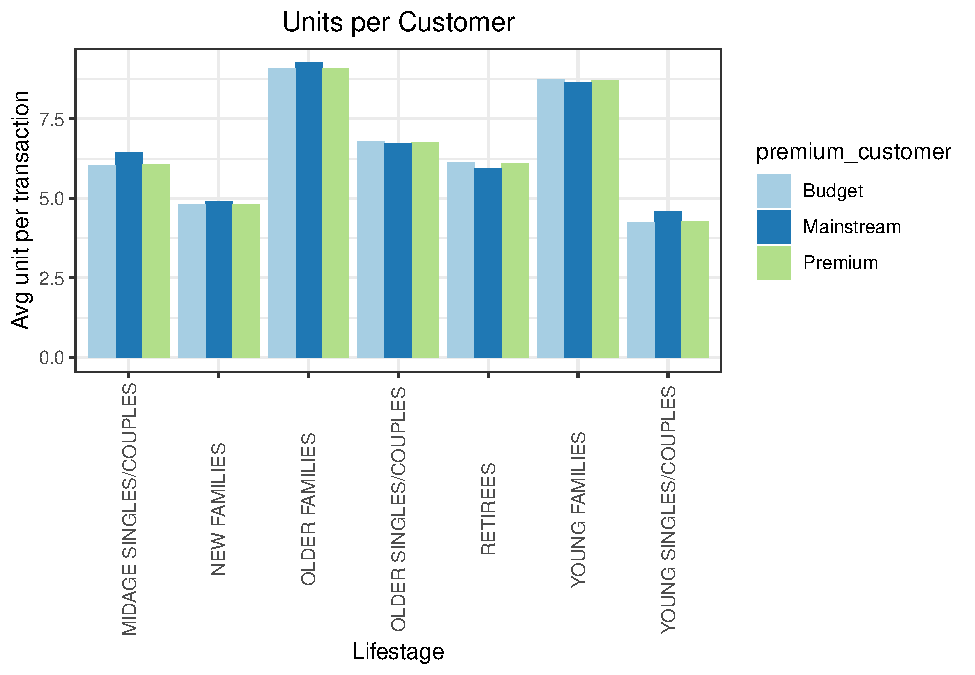
\includegraphics{quantium_analysis_files/figure-latex/unnamed-chunk-33-1.pdf}
Older families and young families in general buy more chips per
customer.

Investigate the average price per unit chips bought for each customer
segment as this is also a driver of total sales. \#\#\#\# Average price
per unit by lifestage and premium\_customer

\begin{Shaded}
\begin{Highlighting}[]
\NormalTok{all\_data }\SpecialCharTok{\%\textgreater{}\%}
  \FunctionTok{group\_by}\NormalTok{(lifestage, premium\_customer) }\SpecialCharTok{\%\textgreater{}\%}
  \FunctionTok{summarize}\NormalTok{(}\AttributeTok{avg\_price =} \FunctionTok{sum}\NormalTok{(tot\_sales)}\SpecialCharTok{/}\FunctionTok{sum}\NormalTok{(prod\_qty)) }\SpecialCharTok{\%\textgreater{}\%}
  \FunctionTok{arrange}\NormalTok{(}\FunctionTok{desc}\NormalTok{(avg\_price))}
\end{Highlighting}
\end{Shaded}

\begin{verbatim}
## `summarise()` has grouped output by 'lifestage'. You can override using the
## `.groups` argument.
\end{verbatim}

\begin{verbatim}
## # A tibble: 21 x 3
## # Groups:   lifestage [7]
##    lifestage              premium_customer avg_price
##    <chr>                  <chr>                <dbl>
##  1 YOUNG SINGLES/COUPLES  Mainstream            4.07
##  2 MIDAGE SINGLES/COUPLES Mainstream            3.99
##  3 NEW FAMILIES           Mainstream            3.94
##  4 RETIREES               Budget                3.93
##  5 NEW FAMILIES           Budget                3.93
##  6 RETIREES               Premium               3.92
##  7 OLDER SINGLES/COUPLES  Premium               3.90
##  8 OLDER SINGLES/COUPLES  Budget                3.89
##  9 NEW FAMILIES           Premium               3.89
## 10 RETIREES               Mainstream            3.85
## # i 11 more rows
\end{verbatim}

\hypertarget{create-a-plot-3}{%
\paragraph{Create a plot}\label{create-a-plot-3}}

\begin{Shaded}
\begin{Highlighting}[]
\NormalTok{avg\_price\_by\_segment }\OtherTok{\textless{}{-}}\NormalTok{ all\_data }\SpecialCharTok{\%\textgreater{}\%}
  \FunctionTok{group\_by}\NormalTok{(lifestage, premium\_customer) }\SpecialCharTok{\%\textgreater{}\%}
  \FunctionTok{summarize}\NormalTok{(}\AttributeTok{avg\_price =} \FunctionTok{sum}\NormalTok{(tot\_sales)}\SpecialCharTok{/}\FunctionTok{sum}\NormalTok{(prod\_qty)) }\SpecialCharTok{\%\textgreater{}\%}
  \FunctionTok{arrange}\NormalTok{(}\FunctionTok{desc}\NormalTok{(avg\_price))}
\end{Highlighting}
\end{Shaded}

\begin{verbatim}
## `summarise()` has grouped output by 'lifestage'. You can override using the
## `.groups` argument.
\end{verbatim}

\begin{Shaded}
\begin{Highlighting}[]
\CommentTok{\# Plotting the results}
\FunctionTok{ggplot}\NormalTok{(avg\_price\_by\_segment, }\FunctionTok{aes}\NormalTok{(}\AttributeTok{x =}\NormalTok{ lifestage, }\AttributeTok{y =}\NormalTok{ avg\_price, }\AttributeTok{fill =}\NormalTok{ premium\_customer)) }\SpecialCharTok{+}
  \FunctionTok{geom\_bar}\NormalTok{(}\AttributeTok{stat =} \StringTok{"identity"}\NormalTok{, }\AttributeTok{position =} \StringTok{"dodge"}\NormalTok{) }\SpecialCharTok{+}
  \FunctionTok{labs}\NormalTok{(}\AttributeTok{title =} \StringTok{"Price per Unit"}\NormalTok{,}
       \AttributeTok{x =} \StringTok{"Lifestage"}\NormalTok{,}
       \AttributeTok{y =} \StringTok{"Avg price per unit"}\NormalTok{) }\SpecialCharTok{+}
  \FunctionTok{theme}\NormalTok{(}\AttributeTok{axis.text.x=} \FunctionTok{element\_text}\NormalTok{(}\AttributeTok{angle=}\DecValTok{90}\NormalTok{,}\AttributeTok{vjust=}\FloatTok{0.5}\NormalTok{))}\SpecialCharTok{+}
  \FunctionTok{scale\_fill\_brewer}\NormalTok{(}\AttributeTok{palette =} \StringTok{"Paired"}\NormalTok{)}
\end{Highlighting}
\end{Shaded}

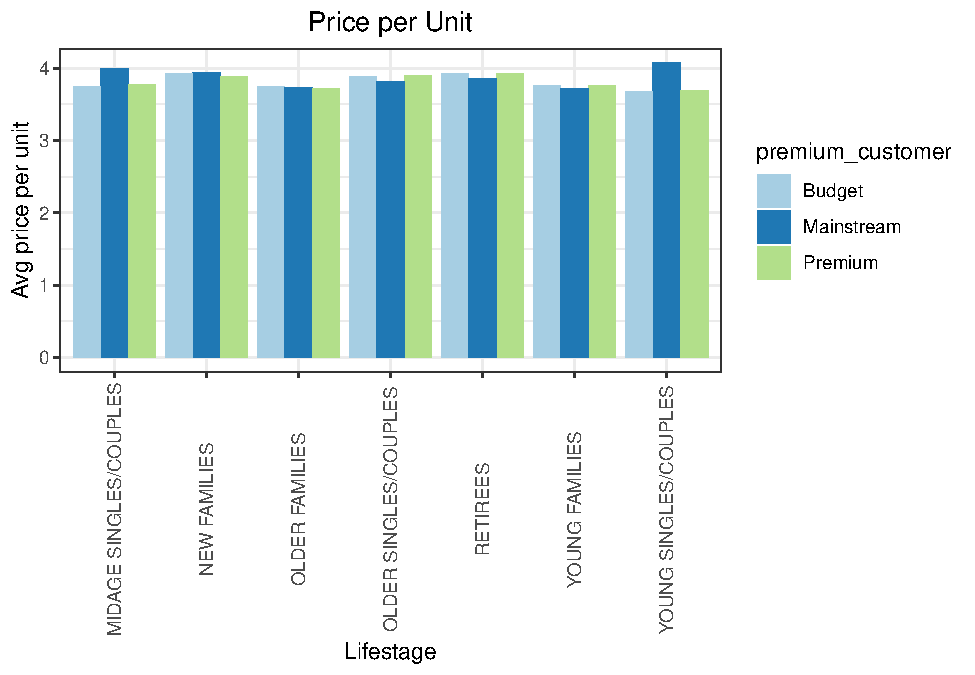
\includegraphics{quantium_analysis_files/figure-latex/unnamed-chunk-35-1.pdf}
Mainstream midage and young singles and couples are more willing to pay
more per packet of chips compared to their budget and premium
counterparts. This may be due to premium shoppers being more likely to
buy healthy snacks and when they buy chips, this is mainly for
entertainment purposes rather than their own consumption. This is also
supported by there being fewer premium midage and young singles and
couples buying chips compared to their mainstream counterparts.

As the difference in average price per unit isn't large, we can check if
this difference is statistically different. \#\#\#\# Perform an
independent t-test between mainstream vs premium and budget midage and
young singles and couples

\begin{Shaded}
\begin{Highlighting}[]
\FunctionTok{setDT}\NormalTok{(all\_data)}
\NormalTok{price\_per\_unit }\OtherTok{\textless{}{-}}\NormalTok{ all\_data[, price }\SpecialCharTok{:=}\NormalTok{ tot\_sales}\SpecialCharTok{/}\NormalTok{prod\_qty]}
\FunctionTok{t.test}\NormalTok{(all\_data[lifestage }\SpecialCharTok{\%in\%} \FunctionTok{c}\NormalTok{(}\StringTok{"YOUNG SINGLES/COUPLES"}\NormalTok{, }\StringTok{"MIDAGE SINGLES/COUPLES"}\NormalTok{) }\SpecialCharTok{\&}\NormalTok{ premium\_customer }\SpecialCharTok{==} \StringTok{"Mainstream"}\NormalTok{, price]}
\NormalTok{, all\_data[lifestage }\SpecialCharTok{\%in\%} \FunctionTok{c}\NormalTok{(}\StringTok{"YOUNG SINGLES/COUPLES"}\NormalTok{, }\StringTok{"MIDAGE SINGLES/COUPLES"}\NormalTok{) }\SpecialCharTok{\&}\NormalTok{ premium\_customer }\SpecialCharTok{!=} \StringTok{"Mainstream"}\NormalTok{, price]}
\NormalTok{, }\AttributeTok{alternative =} \StringTok{"greater"}\NormalTok{)}
\end{Highlighting}
\end{Shaded}

\begin{verbatim}
## 
##  Welch Two Sample t-test
## 
## data:  all_data[lifestage %in% c("YOUNG SINGLES/COUPLES", "MIDAGE SINGLES/COUPLES") & premium_customer == "Mainstream", price] and all_data[lifestage %in% c("YOUNG SINGLES/COUPLES", "MIDAGE SINGLES/COUPLES") & premium_customer != "Mainstream", price]
## t = 37.624, df = 54791, p-value < 2.2e-16
## alternative hypothesis: true difference in means is greater than 0
## 95 percent confidence interval:
##  0.3187234       Inf
## sample estimates:
## mean of x mean of y 
##  4.039786  3.706491
\end{verbatim}

The t-test results in a p-value of 2.2e-16, i.e.~the unit price for
mainstream, young and mid-age singles and couples ARE significantly
higher than that of budget or premium, young and midage singles and
couples.

\hypertarget{deep-dive-into-specific-customer-segments-for-insights}{%
\subsection{Deep dive into specific customer segments for
insights}\label{deep-dive-into-specific-customer-segments-for-insights}}

We might want to target customer segments that contribute the most to
sales to retain them or further increase sales. Let's look at Mainstream
- young singles/couples. For instance, let's find out if they tend to
buy a particular brand of chips.

\hypertarget{deep-dive-into-mainstream-young-singlescouples}{%
\paragraph{Deep dive into Mainstream, young
singles/couples}\label{deep-dive-into-mainstream-young-singlescouples}}

\begin{Shaded}
\begin{Highlighting}[]
\NormalTok{segment\_1 }\OtherTok{\textless{}{-}}\NormalTok{ all\_data[all\_data}\SpecialCharTok{$}\NormalTok{lifestage }\SpecialCharTok{==} \StringTok{"YOUNG SINGLES/COUPLES"} \SpecialCharTok{\&}\NormalTok{ all\_data}\SpecialCharTok{$}\NormalTok{premium\_customer }\SpecialCharTok{==}\StringTok{"Mainstream"}\NormalTok{,]}
\NormalTok{other }\OtherTok{\textless{}{-}}\NormalTok{ all\_data[}\SpecialCharTok{!}\NormalTok{(all\_data}\SpecialCharTok{$}\NormalTok{lifestage }\SpecialCharTok{==} \StringTok{"YOUNG SINGLES/COUPLES"} \SpecialCharTok{\&}\NormalTok{ all\_data}\SpecialCharTok{$}\NormalTok{premium\_customer }\SpecialCharTok{==}\StringTok{"Mainstream"}\NormalTok{),]}
\end{Highlighting}
\end{Shaded}

\hypertarget{brand-affinity-compared-to-the-rest-of-the-population}{%
\paragraph{Brand affinity compared to the rest of the
population}\label{brand-affinity-compared-to-the-rest-of-the-population}}

\begin{Shaded}
\begin{Highlighting}[]
\CommentTok{\# Calculate total quantities}
\NormalTok{quantity\_segment1 }\OtherTok{\textless{}{-}}\NormalTok{ segment\_1[, }\FunctionTok{sum}\NormalTok{(segment\_1}\SpecialCharTok{$}\NormalTok{prod\_qty)]}
\NormalTok{quantity\_other }\OtherTok{\textless{}{-}}\NormalTok{ other[, }\FunctionTok{sum}\NormalTok{(other}\SpecialCharTok{$}\NormalTok{prod\_qty)]}

\CommentTok{\# Calculate brand proportions for each segment}
\NormalTok{quantity\_segment1\_by\_brand }\OtherTok{\textless{}{-}}\NormalTok{ segment\_1[, .(}\AttributeTok{target\_segment =} \FunctionTok{sum}\NormalTok{(prod\_qty)}\SpecialCharTok{/}\NormalTok{quantity\_segment1), by }\OtherTok{=}\NormalTok{ brand]}
\NormalTok{quantity\_other\_by\_brand }\OtherTok{\textless{}{-}}\NormalTok{ other[, .(}\AttributeTok{other =} \FunctionTok{sum}\NormalTok{(prod\_qty)}\SpecialCharTok{/}\NormalTok{quantity\_other), by }\OtherTok{=}\NormalTok{ brand]}

\CommentTok{\# Merge brand proportions}
\NormalTok{brand\_proportions }\OtherTok{\textless{}{-}} \FunctionTok{merge}\NormalTok{(quantity\_segment1\_by\_brand,quantity\_other\_by\_brand)[, affinityToBrand }\SpecialCharTok{:=}\NormalTok{ target\_segment}\SpecialCharTok{/}\NormalTok{other]}

\CommentTok{\# Order by affinityToBrand}
\NormalTok{brand\_proportions[}\FunctionTok{order}\NormalTok{(}\SpecialCharTok{{-}}\NormalTok{affinityToBrand)]}
\end{Highlighting}
\end{Shaded}

\begin{verbatim}
##          brand target_segment       other affinityToBrand
##  1:   TYRRELLS    0.031552795 0.025692464       1.2280953
##  2:   TWISTIES    0.046183575 0.037876520       1.2193194
##  3:    DORITOS    0.122760524 0.101074684       1.2145526
##  4:     KETTLE    0.197984817 0.165553442       1.1958967
##  5:   TOSTITOS    0.045410628 0.037977861       1.1957131
##  6:   PRINGLES    0.119420290 0.100634769       1.1866703
##  7:       COBS    0.044637681 0.039048861       1.1431238
##  8:  INFUZIONS    0.064679089 0.057064679       1.1334347
##  9:      THINS    0.060372671 0.056986370       1.0594230
## 10:    GRNWVES    0.032712215 0.031187957       1.0488733
## 11:   CHEEZELS    0.017971014 0.018646902       0.9637534
## 12:     SMITHS    0.096369910 0.124583692       0.7735355
## 13:     FRENCH    0.003947550 0.005758060       0.6855694
## 14:    CHEETOS    0.008033126 0.012066591       0.6657329
## 15:        RRD    0.043809524 0.067493678       0.6490908
## 16:    NATURAL    0.019599724 0.030853989       0.6352412
## 17:        CCS    0.011180124 0.018895650       0.5916771
## 18:   SUNBITES    0.006349206 0.012580210       0.5046980
## 19: WOOLWORTHS    0.024099379 0.049427188       0.4875733
## 20:     BURGER    0.002926156 0.006596434       0.4435967
\end{verbatim}

We can see that : * Mainstream young singles/couples are 25\% more
likely to purchase Tyrrells chips compared to the rest of the population
* Mainstream young singles/couples are 65\% less likely to purchase
Burger Rings compared to the rest of the population

\end{document}
